\documentclass[times,review]{article}

\usepackage{framed,multirow}
\usepackage{booktabs}
\usepackage[usenames, dvipsnames, svgnames]{xcolor}
\usepackage{tikz}
\usepackage{pgfplots}
\usepackage{fontawesome}
\usepackage{amssymb}
\usepackage{latexsym}
\usepackage{url}
\usepackage{longtable}
\usepackage[colorlinks]{hyperref}
\usepackage{subcaption}
\usepackage{float}
\usepackage{listings}
\usepackage{xspace}
\usepackage[margin=2cm]{geometry}
\usepackage{amsmath}

\newcommand{\ie}{i.e\@.\xspace}
\newcommand{\eg}{e.g\@.\xspace}
\newcommand{\etal}{et al\@.\xspace}

\title{
    Encryption agnostic classifiers of traffic originators and\\their application to anomaly detection\\
    {\Large Traffic statistics dataset and insights on machine learning models}
}
\author{
    Daniele Canavese$^\text{a}$\\\href{mailto:daniele.canavese@polito.it}{daniele.canavese@polito.it}\and
    Leonardo Regano$^\text{a}$\\\href{leonardo.regano@polito.it}{leonardo.regano@polito.it}\and
    Cataldo Basile$^\text{a}$\\\href{cataldo.basile@polito.it}{cataldo.basile@polito.it}\and
    Gabriele Ciravegna$^\text{b}$\\\href{gabriele.ciravegna@unifi.it}{gabriele.ciravegna@unifi.it}\and
    Antonio Lioy$^\text{a}$\\\href{lioy@polito.it}{lioy@polito.it}
}
\date{}

\begin{document}
\maketitle
\begin{flushleft}
    $^\text{a}$ Dipartimento di Automatica e Informatica, Politecnico di Torino, 10129 Torino, Italy\\
    $^\text{b}$ Dipartimento di Ingegneria dell'Informazione, Università degli Studi di Firenze, 53100 Siena, Italy
\end{flushleft}
\newpage
\section*{Data set}

This section reports several statistics about the data set. Table~\ref{tab:tools} lists the tools that have been used to generate the traffic that has been considered in the presented
data set.
Table~\ref{tab:features} reports the features that have been used to train and test the machine-learning
models.

\begin{table}[H]
    \centering
    \begin{tabular}{llcc}
         \toprule
         \textsc{application} & \textsc{category} & \textsc{Windows} & \textsc{Linux}\\
         \midrule
         Chrome 48                        & browser               & \faCheckCircle           & \faCheckCircle\\
         Chrome 68                        & browser               & \faCheckCircle           & \faCheckCircle\\
         Firefox 42                       & browser               & \faCheckCircle           & \faCheckCircle\\
         Firefox 62                       & browser               & \faCheckCircle           & \faCheckCircle\\
         {Firefox 68          }           & {browser}     & {\faCircleO}     & {\faCheckCircle}\\
         Edge 42                          & browser               & \faCheckCircle           & \faCircleO\\
         {Opera 62}                      & {browser}     & {\faCheckCircle} & {\faCircleO}\\
         \cmidrule(lr){1-4}
         GoldenEye 3.49.2               & stress tool           & \faCheckCircle           & \faCheckCircle\\
         HULK 1.0                       & stress tool           & \faCheckCircle           & \faCheckCircle\\
         {RudyJS 1.0.0}         & {stress tool} & {\faCheckCircle} & {\faCheckCircle}\\
         {SlowHTTPTest 1.6}     & {stress tool} & {\faCircleO}     & {\faCheckCircle}\\
         SlowLoris 7.70                 & stress tool           & \faCheckCircle           & \faCheckCircle\\
          \cmidrule(lr){1-4}
        Curl 7.55                      & web crawler           & \faCheckCircle           & \faCheckCircle\\
         {GrabSite 2.1.16}      & {web crawler} & {\faCircleO}     & {\faCheckCircle}\\
         Httrack 3.49.2                 & web crawler           & \faCheckCircle           & \faCheckCircle\\
         Wget 1.19                      & web crawler           & \faCheckCircle           & \faCheckCircle\\
         {Wpull 2.0.1}          & {web crawler} & {\faCheckCircle} & {\faCheckCircle}\\
        \bottomrule
    \end{tabular}
    \caption{Tools used to generate the traffic considered in the experiments.}
    \label{tab:tools}
\end{table}

\begin{table}[H]
    \centering
    \begin{tabular}{lll}
        \toprule
        & \textsc{feature} & \textsc{unit}\\
        \midrule
        1 &\# packets (both directions) & $packets$\\
        2 &\# packets with payload (both directions) & $packets$\\
        3 &\# retransmitted packets (both directions) & $packets$\\
        4 &\# out of sequence packets (both directions) & $packets$\\
        5 &\# packets with ACK set (both directions) & $packets$\\
        6 &\# packets with ACK set and no payload (both directions) & $packets$\\
        7 &\# packets with FIN set (both directions) & $packets$\\
        8 &\# packets with RST set (both directions)\footnotemark & $packets$\\
        9 &\# packets with SYN set (both directions) & $packets$\\

        10 &\# payload bytes excluding retransmissions (both directions) & $bytes$\\
        11 &\# payload bytes including retransmissions (both directions) & $bytes$\\
        12 & \# retransmitted bytes (both directions) & $bytes$\\

        13& flow duration & $ms$\\
        14 &relative time of first payload packet (both directions) & $ms$\\
        15 &relative time of last payload packet (both directions) & $ms$\\
        16 &relative time of first ACK packet (both directions) & $ms$\\

        17 &TCP connection correctly terminated & $boolean$\\
        \bottomrule
    \end{tabular}
    \caption{TCP statistics used as classification features.}
    \label{tab:features}
\end{table}

\footnotetext{Actually this can be only 0 or 1 since a proper TCP implementation will reset a connection after receiving a RST packet.}

Finally, several statistics, grouped by labels, are reported: the average number of packets and bytes send by the client or by the server and the average connection duration in milliseconds.
Table~\ref{tab:means_category}, \ref{tab:means_application_short} and \ref{tab:means_application_long} respectively
reports the averages for the three categories (browsers, crawlers and DoS tools), all the tools and their instances in data set.
\begin{table}[H]
	\centering
	\begin{tabular}{lrrrrr}
		\toprule
		 & \multicolumn{2}{c}{\textsc{sent by client}} & \multicolumn{2}{c}{\textsc{sent by server}}\\
		\cmidrule(lr){2-3}
		\cmidrule(lr){4-5}
		\textsc{category} & \textsc{packets} & \textsc{bytes} & \textsc{packets} & \textsc{bytes} & \textsc{duration} [$ms$]\\
		\midrule
		browser & 30.590 & 2381.743 & 41.748 & 46519.913 & 25495.701\\
		crawler & 95.668 & 1568.130 & 158.849 & 344685.003 & 4589.703\\
		dos & 10.974 & 738.409 & 16.329 & 17955.801 & 2895.279\\
		\bottomrule
	\end{tabular}
	\caption{Means of some features for the category in our data set.}
	\label{tab:means_category}
\end{table}

\begin{table}[H]
	\centering
	\begin{tabular}{lrrrrr}
		\toprule
		 & \multicolumn{2}{c}{\textsc{sent by client}} & \multicolumn{2}{c}{\textsc{sent by server}}\\
		\cmidrule(lr){2-3}
		\cmidrule(lr){4-5}
		\textsc{tool} & \textsc{packets} & \textsc{bytes} & \textsc{packets} & \textsc{bytes} & \textsc{duration} [$ms$]\\
		\midrule
		chrome & 30.605 & 2587.957 & 43.548 & 46727.950 & 36023.258\\
		curl & 48.260 & 539.707 & 71.030 & 91280.696 & 608.296\\
		edge & 23.135 & 2024.088 & 21.693 & 21782.879 & 12693.361\\
		firefox & 40.620 & 2744.452 & 60.108 & 71260.752 & 24748.461\\
		goldeneye & 13.061 & 800.137 & 21.071 & 24220.021 & 1409.918\\
		grabsite & 368.901 & 3929.413 & 583.037 & 1803017.128 & 15427.538\\
		httrack & 16.424 & 1009.946 & 21.192 & 23018.443 & 2517.901\\
		hulk & 5.711 & 573.383 & 4.576 & 2659.303 & 5909.654\\
		opera & 25.263 & 1914.553 & 47.881 & 53419.715 & 40428.032\\
		rudy & 11.332 & 713.800 & 10.997 & 3342.403 & 15770.126\\
		slowhttptest & 8.640 & 1406.865 & 6.826 & 3494.015 & 11974.112\\
		slowloris & 5.280 & 164.620 & 3.890 & 47.859 & 13641.368\\
		wget & 129.312 & 2134.542 & 246.652 & 328985.405 & 2756.862\\
		wpull & 115.476 & 1239.060 & 214.299 & 296092.743 & 8558.179\\
		\bottomrule
	\end{tabular}
	\caption{Means of some features for the tool in our data set.}
	\label{tab:means_application_short}
\end{table}

\begin{table}[H]
	\centering
	\begin{tabular}{lrrrrr}
		\toprule
		 & \multicolumn{2}{c}{\textsc{sent by client}} & \multicolumn{2}{c}{\textsc{sent by server}}\\
		\cmidrule(lr){2-3}
		\cmidrule(lr){4-5}
		\textsc{tool instance} & \textsc{packets} & \textsc{bytes} & \textsc{packets} & \textsc{bytes} & \textsc{duration} [$ms$]\\
		\midrule
		chrome-48.0.2564.109 & 31.145 & 2337.780 & 41.950 & 41918.843 & 34469.858\\
		chrome-68.0.3440.84 & 29.843 & 2941.171 & 45.803 & 53517.726 & 38216.437\\
		curl-7.55.1 & 31.203 & 649.631 & 53.382 & 65814.020 & 431.330\\
		curl-7.61.0 & 67.340 & 416.752 & 90.771 & 119766.433 & 806.241\\
		edge-42.17134.1.0 & 23.135 & 2024.088 & 21.693 & 21782.879 & 12693.361\\
		firefox-42.0 & 37.651 & 3162.645 & 57.196 & 66622.033 & 24610.871\\
		firefox-62.0 & 49.066 & 3359.130 & 72.157 & 84900.460 & 33731.822\\
		firefox-68.0 & 30.374 & 1155.053 & 43.732 & 54509.414 & 9834.131\\
		goldeneye-2.1 & 13.061 & 800.137 & 21.071 & 24220.021 & 1409.918\\
		grabsite-2.1.16 & 368.901 & 3929.413 & 583.037 & 1803017.128 & 15427.538\\
		httrack-3.49.2 & 16.424 & 1009.946 & 21.192 & 23018.443 & 2517.901\\
		hulk-1.0 & 5.711 & 573.383 & 4.576 & 2659.303 & 5909.654\\
		opera-62.0.3331.66 & 25.263 & 1914.553 & 47.881 & 53419.715 & 40428.032\\
		rudy-1.0.0 & 11.332 & 713.800 & 10.997 & 3342.403 & 15770.126\\
		slowhttptest-1.6 & 8.640 & 1406.865 & 6.826 & 3494.015 & 11974.112\\
		slowloris-0.1.4 & 5.404 & 164.220 & 3.973 & 48.299 & 13392.927\\
		slowloris-0.1.5 & 5.159 & 165.008 & 3.810 & 47.434 & 13881.584\\
		wget-1.11.4 & 92.605 & 1024.641 & 184.089 & 249312.020 & 2076.603\\
		wget-1.19.5 & 176.123 & 3549.987 & 326.437 & 430592.154 & 3624.391\\
		wpull-2.0.1 & 115.476 & 1239.060 & 214.299 & 296092.743 & 8558.179\\
		\bottomrule
	\end{tabular}
	\caption{Means of some features for the tool instance in our data set.}
	\label{tab:means_application_long}
\end{table}


\section*{Classifiers}

This section reports several statistics and plots about the models for classifying the traffic into various classes.
%
Three different models have been considered for each classification task: a random forest (via the
\texttt{RandomForestClassifier} class in \texttt{scikit-learn}), an extra-trees (via the \texttt{ExtraTreesClassifier}
class in \texttt{scikit-learn}) and a neural network (a custom class implemented in \texttt{PyTorch} and
\texttt{skorch}).
The optimization process was performed using the \texttt{hyperopt} package using a Bayesian
optimization procedure.

For each classifier, the following data are reported:
\begin{itemize}
    \item the plots showing the values of the $R_k$ statistics as our Bayesian hyper-parameters optimization process
    progressed (Figs.~\ref{fig:optimization_category_random_forest}, \ref{fig:optimization_category_extra_trees},
    \ref{fig:optimization_category_neural_network}, \ref{fig:optimization_application_short_random_forest},
    \ref{fig:optimization_application_short_extra_trees}, \ref{fig:optimization_application_short_neural_network},
    \ref{fig:optimization_application_long_random_forest}, \ref{fig:optimization_application_long_extra_trees} and
    \ref{fig:optimization_application_long_neural_network});
    \item the tables listing the optimal hyper-parameters found by our Bayesian optimization process
    (Tables~\ref{tab:hyperparameters_category_random_forest}, \ref{tab:hyperparameters_category_extra_trees},
    \ref{tab:hyperparameters_category_neural_network}, \ref{tab:hyperparameters_application_short_random_forest},
    \ref{tab:hyperparameters_application_short_extra_trees}, \ref{tab:hyperparameters_application_short_neural_network},
    \ref{tab:hyperparameters_application_long_random_forest}, \ref{tab:hyperparameters_application_long_extra_trees}
    and \ref{tab:hyperparameters_application_long_neural_network}) -- we normally used the default values for the
    hyper-parameters not reported\footnote{The most notable exceptions are given by the neural networks' batch size and
    number of epochs, that we chose to set to 1024 and 50, respectively.};
    \item the tables reporting several classification statistics computed on the training set, development set, known
    tools test Set and unknown tools test set (Tables~\ref{tab:classification_category_random_forest},
    \ref{tab:classification_category_extra_trees}, \ref{tab:classification_category_neural_network},
    \ref{tab:classification_application_short_random_forest}, \ref{tab:classification_application_short_extra_trees},
    \ref{tab:classification_application_short_neural_network}, \ref{tab:classification_application_long_random_forest},
    \ref{tab:classification_application_long_extra_trees} and \ref{tab:classification_application_long_neural_network});
    \item the confusion matrices for each classifier (Tables.~\ref{tab:confusion_category_random_forest},
    \ref{tab:confusion_category_extra_trees}, \ref{tab:confusion_category_neural_network},
    \ref{tab:confusion_application_short_random_forest}, \ref{tab:confusion_application_short_extra_trees},
    \ref{tab:confusion_application_short_neural_network}, \ref{tab:confusion_application_long_random_forest},
    \ref{tab:confusion_application_long_extra_trees} and \ref{tab:confusion_application_long_neural_network});
    \item the plots depicting how the balanced accuracy changes as the number of exchanged packets increases
    (Figs.~\ref{fig:packets_category_random_forest}, \ref{fig:packets_category_extra_trees},
    \ref{fig:packets_category_neural_network}, \ref{fig:packets_application_short_random_forest},
    \ref{fig:packets_application_short_extra_trees}, \ref{fig:packets_application_short_neural_network},
    \ref{fig:packets_application_long_random_forest}, \ref{fig:packets_application_long_extra_trees} and
    \ref{fig:packets_application_long_neural_network});
    \item the results of the classification of the unknown tools (Tables~\ref{tab:unknown_category_random_forest},
    \ref{tab:unknown_category_extra_trees}, \ref{tab:unknown_category_neural_network},
    \ref{tab:unknown_application_short_random_forest}, \ref{tab:unknown_application_short_extra_trees},
    \ref{tab:unknown_application_short_neural_network}, \ref{tab:unknown_application_long_random_forest},
    \ref{tab:unknown_application_long_extra_trees} and \ref{tab:unknown_application_long_neural_network}).
\end{itemize}

\subsection*{Category classifiers}

This section reports several statistics and plots about the models for classifying the traffic into categories
(e.g. \textsc{browser}, \textsc{crawler} and \textsc{dos} a.k.a. network stress tools).
\begin{figure}[H]
	\centering
	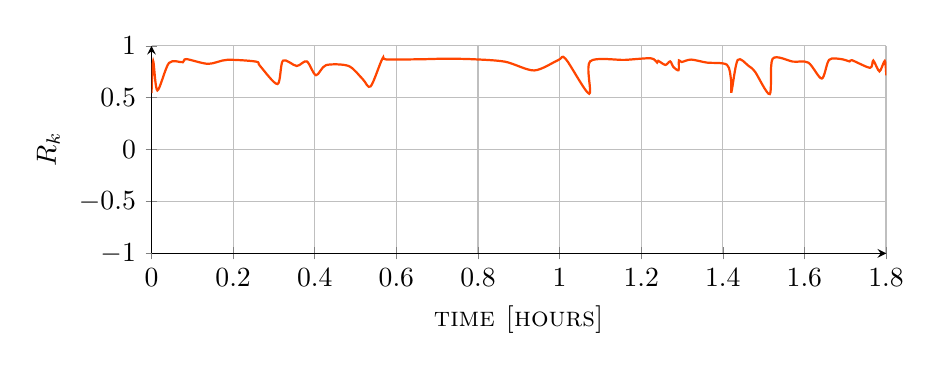
\begin{tikzpicture}
		\begin{axis}[xlabel=\textsc{time [hours]}, ylabel=\textsc{$R_k$}, axis lines=left, grid=major, width=0.9\linewidth, height=12em, ymax=1, ymin=-1]
			\addplot +[mark=none, OrangeRed, thick, smooth] table {
				0.0 0.5444961087808939
				0.004123611111111111 0.8511537523863583
				0.014372777777777778 0.5698992049269191
				0.04273444444444444 0.8343897290417408
				0.0768911111111111 0.8420760152871233
				0.08518444444444444 0.8720495595978613
				0.1388125 0.8261894646121312
				0.1851913888888889 0.8647541227129498
				0.2556111111111111 0.8480853222797268
				0.2658975 0.8060343441693703
				0.30876583333333335 0.6314028702965143
				0.32202416666666667 0.8571194077490936
				0.35565861111111113 0.8056351236685689
				0.3804983333333334 0.8500353157544382
				0.40297805555555555 0.7166104670945992
				0.4277680555555555 0.8138154044494291
				0.4829122222222222 0.8057550379098798
				0.51748 0.6794566906676353
				0.5370322222222222 0.6090771980973686
				0.5658177777777778 0.8761208672966857
				0.576466111111111 0.8672553755060747
				0.661583888888889 0.8705752127728053
				0.7201791666666667 0.8756231672197796
				0.7876677777777777 0.8707195219011391
				0.8665727777777777 0.8467565915633849
				0.9376275 0.7627236065746218
				0.9966172222222223 0.862060541044936
				1.0146355555555555 0.8752327058794888
				1.072577222222222 0.5382420926474235
				1.0748411111111111 0.8500503513023147
				1.1602050000000002 0.8644253104569336
				1.2235383333333334 0.8796329750244695
				1.2390402777777778 0.8385568338949455
				1.2416858333333334 0.8552891635030724
				1.2592969444444444 0.8158802457284906
				1.2711222222222223 0.8507323159260161
				1.2781972222222222 0.7998536171046322
				1.2914630555555555 0.7643073894042848
				1.2925022222222222 0.859163337005119
				1.2991336111111111 0.8438732544884482
				1.3223772222222223 0.8673012928378777
				1.3605297222222223 0.8384795432300679
				1.410015277777778 0.8179457028540305
				1.420321388888889 0.6643935940130762
				1.4213269444444445 0.5576689836005811
				1.436411388888889 0.8633325091985307
				1.4630463888888887 0.8069793168229261
				1.4794466666666666 0.747253453002513
				1.5151569444444444 0.5348611407238524
				1.5221622222222222 0.8751174506904024
				1.5722874999999998 0.847666981150265
				1.6098002777777778 0.8372189474100846
				1.6425980555555555 0.6849397502111092
				1.6605197222222223 0.8644031385554191
				1.6898397222222221 0.8721161602009476
				1.7107966666666667 0.8497743934293334
				1.716603888888889 0.8612318359681981
				1.7608688888888888 0.7879840626524268
				1.7688858333333333 0.8577422363343189
				1.783848611111111 0.7537154075635912
				1.796906111111111 0.8538259300513192
				1.800613611111111 0.71603006988279
			};
		\end{axis}
	\end{tikzpicture}
	\caption{Hyper-parameters optimization plot for the category classifier based on random forest.}
	\label{fig:optimization_category_random_forest}
\end{figure}
\begin{table}[H]
	\centering
	\begin{tabular}{ll}
		\toprule
		\textsc{hyper-parameter} & \textsc{value}\\
		\midrule
		\verb|criterion| & entropy\\
		\verb|max_depth| & 17\\
		\verb|min_samples_leaf| & 9\\
		\verb|min_samples_split| & 38\\
		\verb|n_estimators| & 89\\
		\bottomrule
	\end{tabular}
	\caption{Optimal hyper-parameters for the category classifier based on random forest.}
	\label{tab:hyperparameters_category_random_forest}
\end{table}
\begin{table}[H]
	\centering
	\begin{tabular}{lrrrr}
		\toprule
		\textsc{statistic} & \textsc{training set} & \textsc{dev set} & \textsc{kts} & \textsc{uts}\\
		\midrule
		samples & 955872 & 119484 & 119485 & 30144\\
		accuracy [$\%$] & 97.702 & 97.542 & 97.447 & 40.459\\
		balanced accuracy [$\%$] & 95.568 & 93.997 & 94.041 & 34.031\\
		precision [$\%$] & 86.660 & 85.637 & 85.226 & 32.723\\
		recall [$\%$] & 95.568 & 93.997 & 94.041 & 34.031\\
		Cohen’s kappa [$\%$] & 86.105 & 85.021 & 84.577 & 1.097\\
		F-score [$\%$] & 90.719 & 89.459 & 89.230 & 32.151\\
		Jaccard score [$\%$] & 83.556 & 81.607 & 81.255 & 20.631\\
		Hamming loss & 0.023 & 0.025 & 0.026 & 0.595\\
		zero-one loss & 0.023 & 0.025 & 0.026 & 0.595\\
		$R_k$ & 0.865 & 0.854 & 0.850 & 0.011\\
		\bottomrule
	\end{tabular}
	\caption{Classification statistics for the category classifier based on random forest.}
	\label{tab:classification_category_random_forest}
\end{table}
\begin{table}[H]
	\centering
	\begin{tabular}{ll|lll}
	\setlength{\tabcolsep}{2pt}
		 & & \multicolumn{3}{c}{\textsc{inferred}}\\
		 & & \textsc{browser} & \textsc{crawler} & \textsc{dos}\\
		\midrule
		\multirow{3}{*}{\rotatebox{90}{\textsc{target}}} & \textsc{browser} & 6872 & 194 & 322\\
		 & \textsc{crawler} & 120 & 2112 & 83\\
		 & \textsc{dos} & 1980 & 352 & 107450\\
	\end{tabular}
	\caption{Confusion matrix for the category classifier based on random forest on the KTS.}
	\label{tab:confusion_category_random_forest}
\end{table}
\begin{figure}[H]
	\centering
	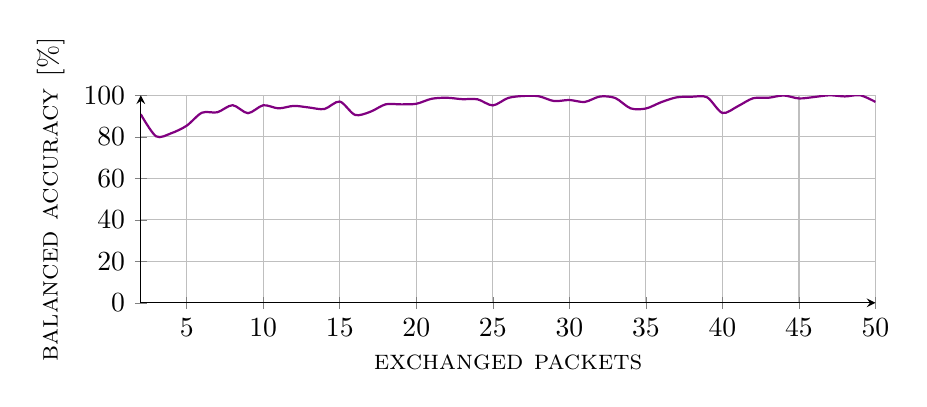
\begin{tikzpicture}
		\begin{axis}[xlabel=\textsc{exchanged packets}, ylabel=\textsc{balanced accuracy [$\%$]}, axis lines=left, grid=major, width=0.9\linewidth, height=12em, ymax=100, ymin=0]
			\addplot +[mark=none, Purple, thick, smooth] table {
				2.0 90.8437826541275
				3.0 80.22175923387613
				4.0 81.73344753465695
				5.0 85.34596811183296
				6.0 91.61303468636976
				7.0 91.80203057112627
				8.0 95.22640971038501
				9.0 91.36070369341854
				10.0 95.18327396668766
				11.0 93.69135587802938
				12.0 94.88908595630309
				13.0 94.09857175822907
				14.0 93.38543917982406
				15.0 96.98121997025248
				16.0 90.53792623521225
				17.0 92.05342784456396
				18.0 95.64432518427675
				19.0 95.61846816545979
				20.0 95.89701398185333
				21.0 98.31200657023261
				22.0 98.80517842038108
				23.0 98.12352459411284
				24.0 98.05082070707071
				25.0 95.12037669932405
				26.0 98.70064967516242
				27.0 99.66996699669967
				28.0 99.53569680441929
				29.0 97.21638655462185
				30.0 97.72358218649778
				31.0 96.77767052767052
				32.0 99.41117240171614
				33.0 98.6711395433505
				34.0 93.70096697682904
				35.0 93.62114076399791
				36.0 96.66879445442113
				37.0 98.98848428260193
				38.0 99.30555555555554
				39.0 99.0135468396338
				40.0 91.4850136239782
				41.0 94.70026727758687
				42.0 98.55776306107433
				43.0 98.79120879120879
				44.0 99.89451476793249
				45.0 98.4729064039409
				46.0 99.16666666666667
				47.0 100.0
				48.0 99.4413407821229
				49.0 100.0
				50.0 96.79633867276888
			};
		\end{axis}
	\end{tikzpicture}
	\caption{Balanced accuracy vs. exchange packets plot for the category classifier based on random forest on the KTS.}
	\label{fig:packets_category_random_forest}
\end{figure}
\begin{table}[H]
	\centering
	\begin{subtable}{.45\linewidth}
		\centering
	\begin{tabular}{ll}
		\toprule
		\textsc{inferred class} & \textsc{samples}\\
		\midrule
		browser & 3291\\
		crawler & 2623\\
		dos & 620\\
		\bottomrule
	\end{tabular}
	\caption{Classification of \textsc{firefox-68.0}.}
	\end{subtable}
	\begin{subtable}{.45\linewidth}
		\centering
	\begin{tabular}{ll}
		\toprule
		\textsc{inferred class} & \textsc{samples}\\
		\midrule
		browser & 1369\\
		crawler & 883\\
		dos & 1413\\
		\bottomrule
	\end{tabular}
	\caption{Classification of \textsc{grabsite-2.1.16}.}
	\end{subtable}
	\begin{subtable}{.45\linewidth}
		\centering
	\begin{tabular}{ll}
		\toprule
		\textsc{inferred class} & \textsc{samples}\\
		\midrule
		browser & 6149\\
		crawler & 605\\
		dos & 2196\\
		\bottomrule
	\end{tabular}
	\caption{Classification of \textsc{opera-62.0.3331.66}.}
	\end{subtable}
	\begin{subtable}{.45\linewidth}
		\centering
	\begin{tabular}{ll}
		\toprule
		\textsc{inferred class} & \textsc{samples}\\
		\midrule
		browser & 6657\\
		crawler & 2465\\
		dos & 1873\\
		\bottomrule
	\end{tabular}
	\caption{Classification of \textsc{slowhttptest-1.6}.}
	\end{subtable}
	\caption{Classification of unknown tools for the category classifier based on random forest.}
	\label{tab:unknown_category_random_forest}
\end{table}

\begin{figure}[H]
	\centering
	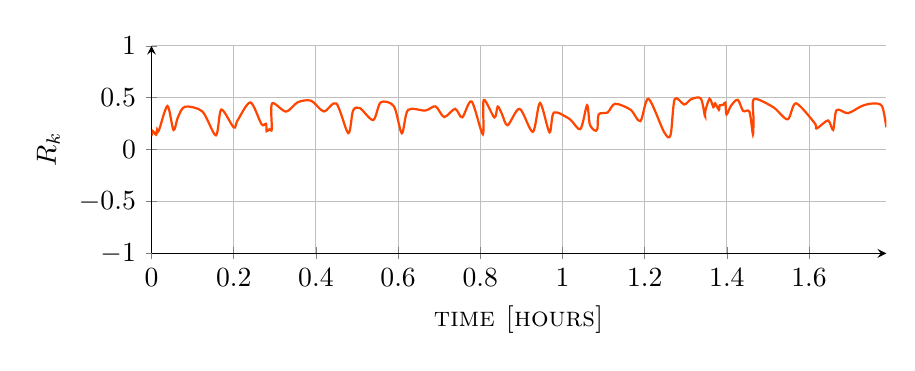
\begin{tikzpicture}
		\begin{axis}[xlabel=\textsc{time [hours]}, ylabel=\textsc{$R_k$}, axis lines=left, grid=major, width=0.9\linewidth, height=12em, ymax=1, ymin=-1]
			\addplot +[mark=none, OrangeRed, thick, smooth] table {
				0.0 0.13135369747917117
				0.0025855555555555554 0.17978227963505983
				0.011065 0.1433706880737134
				0.013418055555555556 0.19059945822298427
				0.017869444444444445 0.1835153962042667
				0.03875805555555555 0.4202933378943818
				0.05345055555555556 0.1889325520806588
				0.06443777777777777 0.31311058973677475
				0.08145416666666667 0.4133930881661661
				0.12378444444444445 0.3669547958847006
				0.15660416666666666 0.13736965312050634
				0.16978138888888888 0.38611082569702654
				0.2001813888888889 0.21295949563893907
				0.20897666666666667 0.2778809466898707
				0.24047916666666666 0.4544524888262656
				0.2677836111111111 0.24383016391240805
				0.27866 0.2488432276112016
				0.27997305555555557 0.17739668799676617
				0.28716250000000004 0.19663401394502
				0.2926694444444444 0.197838982154629
				0.29330999999999996 0.44512835960341024
				0.3273313888888889 0.36618504872674407
				0.3559847222222222 0.4566089407746047
				0.38857138888888887 0.47060581784904165
				0.41923750000000004 0.3675125821824269
				0.44963583333333335 0.4448459674526829
				0.4787425 0.15837773572161426
				0.4904219444444444 0.3760678380869933
				0.5072680555555555 0.39876745490708554
				0.5393652777777778 0.2848333878185541
				0.5578175 0.45573743056753074
				0.5898619444444445 0.41718393823247857
				0.6091241666666667 0.15702276668836215
				0.6241308333333334 0.38185868928710953
				0.6661866666666666 0.3760794206383165
				0.691013611111111 0.4163915799147428
				0.7121916666666667 0.3135146433415765
				0.7386305555555556 0.3930558510204319
				0.7559472222222222 0.31076940881467824
				0.7788469444444445 0.4641318740787899
				0.8062124999999999 0.14731025238025144
				0.8084169444444445 0.4775649272990927
				0.8342591666666667 0.30928714693435644
				0.8423063888888889 0.4144346955585863
				0.8524380555555555 0.3450651726569078
				0.8665238888888889 0.23489365476101703
				0.8956927777777778 0.3928009008824002
				0.9277994444444444 0.1708045609796094
				0.9453472222222222 0.4488435959844424
				0.9684547222222222 0.16619532461045536
				0.9790966666666667 0.3567234468093689
				1.0172505555555555 0.29484504051138977
				1.043455 0.19719231216543037
				1.0597436111111112 0.4265752170560484
				1.0661752777777778 0.24736387237742072
				1.0772247222222222 0.18623329894253718
				1.0848566666666666 0.19889108753805865
				1.088175 0.33998726409747154
				1.1096827777777778 0.3576138154578811
				1.1280069444444445 0.44145864391484957
				1.1654772222222223 0.3844213178737763
				1.1894377777777776 0.2743321383286894
				1.2092597222222223 0.48955161528378266
				1.2472547222222223 0.16860818228690932
				1.2628700000000002 0.13949046133460127
				1.2730925 0.48651846609553856
				1.2961861111111113 0.4342773809966667
				1.3129688888888889 0.48520954886839207
				1.336426388888889 0.4930517092327974
				1.3466094444444443 0.3210927043016705
				1.3472230555555555 0.36879317618542606
				1.357823888888889 0.4905149879403897
				1.3671708333333332 0.4093075816319852
				1.3712952777777776 0.44611682445826717
				1.3805030555555555 0.38241538947618475
				1.3823174999999999 0.4263812520825596
				1.3907119444444445 0.42999655365252887
				1.3962883333333334 0.45224276816124975
				1.3991397222222224 0.33869879244799456
				1.410311388888889 0.4240680585359524
				1.4263894444444445 0.4799486385900556
				1.4395727777777778 0.3718745708563724
				1.4547747222222223 0.3651755368069844
				1.4633144444444444 0.14737214668233004
				1.4648019444444444 0.2935961842077465
				1.4659758333333333 0.48628746128484934
				1.5129652777777778 0.4081586994466556
				1.5477008333333333 0.2916215600448714
				1.5681469444444445 0.4454973343273979
				1.6138030555555556 0.25359413702740863
				1.6184880555555554 0.2029602655554598
				1.6460261111111112 0.2809671161547638
				1.658562222222222 0.1899507640277969
				1.666983611111111 0.3808328309437742
				1.694725 0.3513901811142677
				1.7280508333333333 0.41954360389996287
				1.7539847222222222 0.4436484824239076
				1.7773955555555554 0.4190367076093213
				1.7877955555555556 0.21566842715213244
			};
		\end{axis}
	\end{tikzpicture}
	\caption{Hyper-parameters optimization plot for the category classifier based on extra-trees.}
	\label{fig:optimization_category_extra_trees}
\end{figure}
\begin{table}[H]
	\centering
	\begin{tabular}{ll}
		\toprule
		\textsc{hyper-parameter} & \textsc{value}\\
		\midrule
		\verb|criterion| & entropy\\
		\verb|max_depth| & 20\\
		\verb|min_samples_leaf| & 3\\
		\verb|min_samples_split| & 37\\
		\verb|n_estimators| & 88\\
		\bottomrule
	\end{tabular}
	\caption{Optimal hyper-parameters for the category classifier based on extra-trees.}
	\label{tab:hyperparameters_category_extra_trees}
\end{table}
\begin{table}[H]
	\centering
	\begin{tabular}{lrrrr}
		\toprule
		\textsc{statistic} & \textsc{training set} & \textsc{dev set} & \textsc{kts} & \textsc{uts}\\
		\midrule
		samples & 955872 & 119484 & 119485 & 30144\\
		accuracy [$\%$] & 85.085 & 85.033 & 85.015 & 37.646\\
		balanced accuracy [$\%$] & 80.692 & 80.216 & 80.373 & 38.510\\
		precision [$\%$] & 62.558 & 62.265 & 62.413 & 33.339\\
		recall [$\%$] & 80.692 & 80.216 & 80.373 & 38.510\\
		Cohen’s kappa [$\%$] & 42.760 & 42.372 & 42.547 & 1.694\\
		F-score [$\%$] & 62.138 & 61.837 & 61.866 & 33.949\\
		Jaccard score [$\%$] & 51.661 & 51.322 & 51.552 & 21.426\\
		Hamming loss & 0.149 & 0.150 & 0.150 & 0.624\\
		zero-one loss & 0.149 & 0.150 & 0.150 & 0.624\\
		$R_k$ & 0.491 & 0.487 & 0.489 & 0.017\\
		\bottomrule
	\end{tabular}
	\caption{Classification statistics for the category classifier based on extra-trees.}
	\label{tab:classification_category_extra_trees}
\end{table}
\begin{table}[H]
	\centering
	\begin{tabular}{ll|lll}
	\setlength{\tabcolsep}{2pt}
		 & & \multicolumn{3}{c}{\textsc{inferred}}\\
		 & & \textsc{browser} & \textsc{crawler} & \textsc{dos}\\
		\midrule
		\multirow{3}{*}{\rotatebox{90}{\textsc{target}}} & \textsc{browser} & 5225 & 1496 & 667\\
		 & \textsc{crawler} & 126 & 1954 & 235\\
		 & \textsc{dos} & 1439 & 13942 & 94401\\
	\end{tabular}
	\caption{Confusion matrix for the category classifier based on extra-trees on the KTS.}
	\label{tab:confusion_category_extra_trees}
\end{table}
\begin{figure}[H]
	\centering
	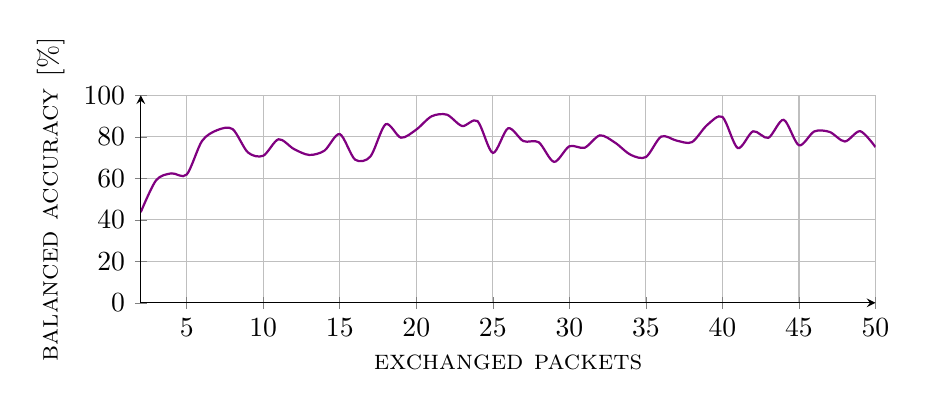
\begin{tikzpicture}
		\begin{axis}[xlabel=\textsc{exchanged packets}, ylabel=\textsc{balanced accuracy [$\%$]}, axis lines=left, grid=major, width=0.9\linewidth, height=12em, ymax=100, ymin=0]
			\addplot +[mark=none, Purple, thick, smooth] table {
				2.0 43.691222570532915
				3.0 59.030648610121176
				4.0 62.37431322090375
				5.0 61.8032169706335
				6.0 77.96059573722181
				7.0 83.21906305576192
				8.0 83.71202582905025
				9.0 72.4771413867778
				10.0 70.86167891470922
				11.0 78.81730045570406
				12.0 74.13348083245074
				13.0 71.2446842703852
				14.0 73.32694532252525
				15.0 81.31408277755185
				16.0 69.00997448387845
				17.0 70.47534074132659
				18.0 86.05512055875252
				19.0 79.5663293873137
				20.0 83.46822475085528
				21.0 89.87217188576273
				22.0 90.64844948459519
				23.0 85.18812930577636
				24.0 87.56313131313132
				25.0 72.2152976022945
				26.0 84.09961685823754
				27.0 77.91341900147461
				28.0 77.34703866862456
				29.0 67.89813486370159
				30.0 75.43031705435797
				31.0 74.73777348777348
				32.0 80.69345941686366
				33.0 77.0947105632704
				34.0 71.32366356504288
				35.0 70.2337345194488
				36.0 80.10717128563243
				37.0 78.16370992841581
				38.0 77.39898989898991
				39.0 85.6612952265126
				40.0 89.56062670299727
				41.0 74.57808323787705
				42.0 82.63428991905813
				43.0 79.48717948717949
				44.0 88.17393342709798
				45.0 75.89490968801314
				46.0 82.57142857142856
				47.0 82.33704829449509
				48.0 77.73671393783125
				49.0 82.6917826917827
				50.0 75.0278706800446
			};
		\end{axis}
	\end{tikzpicture}
	\caption{Balanced accuracy vs. exchange packets plot for the category classifier based on extra-trees on the KTS.}
	\label{fig:packets_category_extra_trees}
\end{figure}
\begin{table}[H]
	\centering
	\begin{subtable}{.45\linewidth}
		\centering
	\begin{tabular}{ll}
		\toprule
		\textsc{inferred class} & \textsc{samples}\\
		\midrule
		browser & 2570\\
		crawler & 1242\\
		dos & 2722\\
		\bottomrule
	\end{tabular}
	\caption{Classification of \textsc{firefox-68.0}.}
	\end{subtable}
	\begin{subtable}{.45\linewidth}
		\centering
	\begin{tabular}{ll}
		\toprule
		\textsc{inferred class} & \textsc{samples}\\
		\midrule
		browser & 837\\
		crawler & 1809\\
		dos & 1019\\
		\bottomrule
	\end{tabular}
	\caption{Classification of \textsc{grabsite-2.1.16}.}
	\end{subtable}
	\begin{subtable}{.45\linewidth}
		\centering
	\begin{tabular}{ll}
		\toprule
		\textsc{inferred class} & \textsc{samples}\\
		\midrule
		browser & 5237\\
		crawler & 1046\\
		dos & 2667\\
		\bottomrule
	\end{tabular}
	\caption{Classification of \textsc{opera-62.0.3331.66}.}
	\end{subtable}
	\begin{subtable}{.45\linewidth}
		\centering
	\begin{tabular}{ll}
		\toprule
		\textsc{inferred class} & \textsc{samples}\\
		\midrule
		browser & 5077\\
		crawler & 4186\\
		dos & 1732\\
		\bottomrule
	\end{tabular}
	\caption{Classification of \textsc{slowhttptest-1.6}.}
	\end{subtable}
	\caption{Classification of unknown tools for the category classifier based on extra-trees.}
	\label{tab:unknown_category_extra_trees}
\end{table}

\begin{figure}[H]
	\centering
	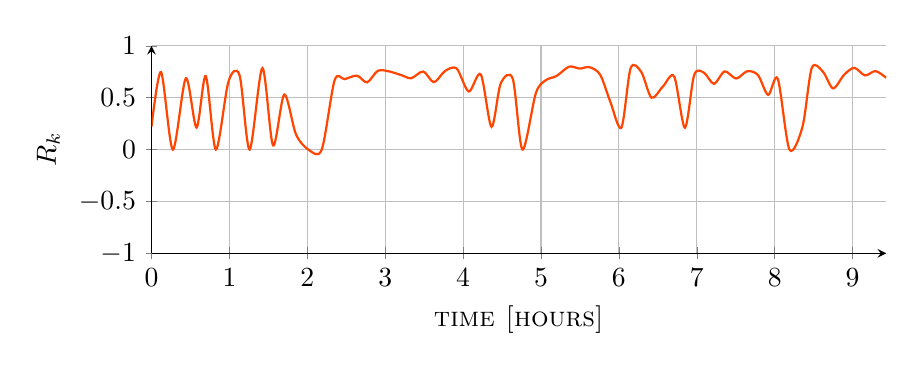
\begin{tikzpicture}
		\begin{axis}[xlabel=\textsc{time [hours]}, ylabel=\textsc{$R_k$}, axis lines=left, grid=major, width=0.9\linewidth, height=12em, ymax=1, ymin=-1]
			\addplot +[mark=none, OrangeRed, thick, smooth] table {
				0.0 0.2210062658266289
				0.12212250000000001 0.7468668542199443
				0.2737058333333333 0.0
				0.44047722222222224 0.6869620634023401
				0.5779966666666667 0.21286318759604017
				0.6963466666666667 0.7077868444361323
				0.8264455555555557 0.0
				0.9877913888888888 0.6553212452037385
				1.1302583333333334 0.7158510962920959
				1.2596577777777778 0.0
				1.4233241666666665 0.78555627833894
				1.560173611111111 0.04031338324190967
				1.7040897222222222 0.5305620645899788
				1.8537841666666666 0.1488366952153271
				2.0139519444444445 0.0
				2.184928888888889 0.0
				2.349692777777778 0.6664427520935514
				2.4791897222222223 0.6790041274095348
				2.637886111111111 0.7123404281741427
				2.7675711111111108 0.6478700713029528
				2.9053605555555557 0.7594913370969733
				3.0537152777777776 0.752626025078389
				3.2100541666666667 0.7165654240441105
				3.3342336111111113 0.6876651438457947
				3.488079722222222 0.7525415707447769
				3.625195833333333 0.6495492115272051
				3.768566111111111 0.7577619062129486
				3.917341388888889 0.7813094792254222
				4.072168055555555 0.5600353040444446
				4.227070277777778 0.7238485747394433
				4.3643025 0.21938184789788054
				4.483167222222222 0.637269512447288
				4.6377825 0.6810954402079779
				4.761978333333333 0.0
				4.9326711111111115 0.5410141600336178
				5.0568905555555554 0.6665433418313889
				5.200257222222222 0.7094159473919907
				5.359889722222222 0.7991117628450763
				5.497729166666667 0.7805775194061032
				5.622027777777777 0.7941215038593585
				5.7592469444444445 0.7218907820667307
				5.888871666666666 0.46286973832844835
				6.0322125 0.21199964894663628
				6.150851111111111 0.7850060226676104
				6.28825138888889 0.746433721275909
				6.418372777777778 0.5000044377566547
				6.566317222222222 0.6093952408434717
				6.7101894444444445 0.7032758499029006
				6.847278888888889 0.21065111766446987
				6.966089444444444 0.7184723832610289
				7.090011944444445 0.7420709094784211
				7.220004444444444 0.6339869249371339
				7.357285555555555 0.7533785641918216
				7.505467222222222 0.6847902950843516
				7.649001944444445 0.7556133453827891
				7.785635277777778 0.717565494444211
				7.9156458333333335 0.5273703354112835
				8.040086666666667 0.6809371503428069
				8.189387777777778 0.0
				8.356989166666667 0.2213466618076342
				8.475808333333333 0.7865802633570821
				8.619317777777779 0.7502291438019768
				8.749226944444445 0.590075638462533
				8.892430833333334 0.7224383394486307
				9.022673055555556 0.7875511127001008
				9.159330277777778 0.7148638548736087
				9.2954025 0.7564852933138435
				9.43203138888889 0.6912593534609529
			};
		\end{axis}
	\end{tikzpicture}
	\caption{Hyper-parameters optimization plot for the category classifier based on neural network.}
	\label{fig:optimization_category_neural_network}
\end{figure}
\begin{table}[H]
	\centering
	\begin{tabular}{ll}
		\toprule
		\textsc{hyper-parameter} & \textsc{value}\\
		\midrule
		\verb|lr| & 0.0027014308955057255\\
		\verb|module__layers| & 4\\
		\verb|module__neurons_per_layer| & 434\\
		\verb|module__p| & 0.1292524544974843\\
		\bottomrule
	\end{tabular}
	\caption{Optimal hyper-parameters for the category classifier based on neural network.}
	\label{tab:hyperparameters_category_neural_network}
\end{table}
\begin{table}[H]
	\centering
	\begin{tabular}{lrrrr}
		\toprule
		\textsc{statistic} & \textsc{training set} & \textsc{dev set} & \textsc{kts} & \textsc{uts}\\
		\midrule
		samples & 955872 & 119484 & 119485 & 30144\\
		accuracy [$\%$] & 96.132 & 96.005 & 96.017 & 41.912\\
		balanced accuracy [$\%$] & 91.123 & 90.207 & 90.308 & 35.058\\
		precision [$\%$] & 75.600 & 74.957 & 74.653 & 33.739\\
		recall [$\%$] & 91.123 & 90.207 & 90.308 & 35.058\\
		Cohen’s kappa [$\%$] & 77.644 & 76.827 & 76.988 & 2.587\\
		F-score [$\%$] & 80.923 & 80.166 & 79.902 & 33.950\\
		Jaccard score [$\%$] & 70.873 & 69.961 & 69.772 & 21.943\\
		Hamming loss & 0.039 & 0.040 & 0.040 & 0.581\\
		zero-one loss & 0.039 & 0.040 & 0.040 & 0.581\\
		$R_k$ & 0.784 & 0.776 & 0.778 & 0.026\\
		\bottomrule
	\end{tabular}
	\caption{Classification statistics for the category classifier based on neural network.}
	\label{tab:classification_category_neural_network}
\end{table}
\begin{table}[H]
	\centering
	\begin{tabular}{ll|lll}
	\setlength{\tabcolsep}{2pt}
		 & & \multicolumn{3}{c}{\textsc{inferred}}\\
		 & & \textsc{browser} & \textsc{crawler} & \textsc{dos}\\
		\midrule
		\multirow{3}{*}{\rotatebox{90}{\textsc{target}}} & \textsc{browser} & 6423 & 489 & 476\\
		 & \textsc{crawler} & 148 & 2018 & 149\\
		 & \textsc{dos} & 1270 & 2227 & 106285\\
	\end{tabular}
	\caption{Confusion matrix for the category classifier based on neural network on the KTS.}
	\label{tab:confusion_category_neural_network}
\end{table}
\begin{figure}[H]
	\centering
	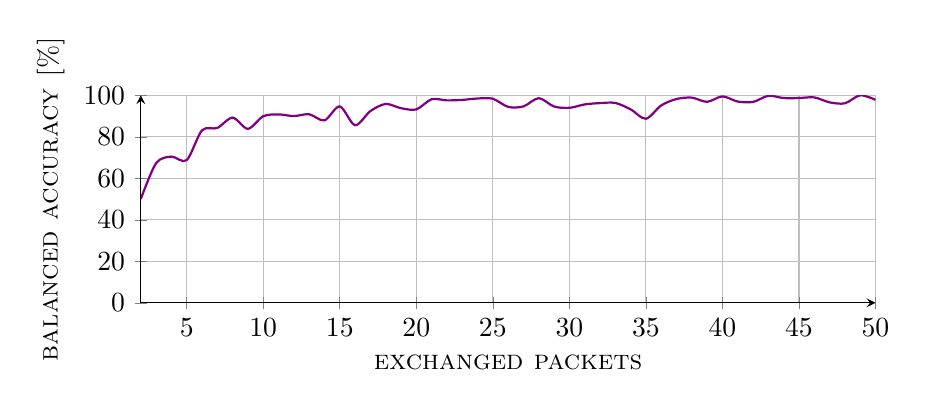
\begin{tikzpicture}
		\begin{axis}[xlabel=\textsc{exchanged packets}, ylabel=\textsc{balanced accuracy [$\%$]}, axis lines=left, grid=major, width=0.9\linewidth, height=12em, ymax=100, ymin=0]
			\addplot +[mark=none, Purple, thick, smooth] table {
				2.0 50.0
				3.0 67.26746714914927
				4.0 70.45817428732478
				5.0 68.73162614056683
				6.0 83.08888313034466
				7.0 84.26442448391528
				8.0 89.24861214775946
				9.0 83.82593657355807
				10.0 89.89600858089419
				11.0 90.78236822880874
				12.0 89.97357623150371
				13.0 90.85193838698513
				14.0 87.9074432369022
				15.0 94.62952849107293
				16.0 85.5770122941313
				17.0 92.36951979858695
				18.0 95.81450967649515
				19.0 93.76805198920685
				20.0 93.1837535326491
				21.0 98.07317331637789
				22.0 97.53939011627072
				23.0 97.76220070337716
				24.0 98.4453914141414
				25.0 98.32424197749276
				26.0 94.41112776944861
				27.0 94.63731479530931
				28.0 98.60709041325782
				29.0 94.5864931338389
				30.0 93.94883557287649
				31.0 95.58719433719433
				32.0 96.22624989055248
				33.0 96.298087758534
				34.0 93.2220397737639
				35.0 88.68480725623583
				36.0 95.10877994444678
				37.0 98.19483348895113
				38.0 98.86363636363636
				39.0 96.8501064153238
				40.0 99.45504087193461
				41.0 96.96830851470027
				42.0 96.79175864606329
				43.0 99.74358974358975
				44.0 98.65994686669791
				45.0 98.65900383141762
				46.0 98.97619047619047
				47.0 96.58899020601149
				48.0 96.13235926085088
				49.0 100.0
				50.0 97.79968315437422
			};
		\end{axis}
	\end{tikzpicture}
	\caption{Balanced accuracy vs. exchange packets plot for the category classifier based on neural network on the KTS.}
	\label{fig:packets_category_neural_network}
\end{figure}
\begin{table}[H]
	\centering
	\begin{subtable}{.45\linewidth}
		\centering
	\begin{tabular}{ll}
		\toprule
		\textsc{inferred class} & \textsc{samples}\\
		\midrule
		browser & 3366\\
		crawler & 358\\
		dos & 2810\\
		\bottomrule
	\end{tabular}
	\caption{Classification of \textsc{firefox-68.0}.}
	\end{subtable}
	\begin{subtable}{.45\linewidth}
		\centering
	\begin{tabular}{ll}
		\toprule
		\textsc{inferred class} & \textsc{samples}\\
		\midrule
		browser & 2012\\
		crawler & 835\\
		dos & 818\\
		\bottomrule
	\end{tabular}
	\caption{Classification of \textsc{grabsite-2.1.16}.}
	\end{subtable}
	\begin{subtable}{.45\linewidth}
		\centering
	\begin{tabular}{ll}
		\toprule
		\textsc{inferred class} & \textsc{samples}\\
		\midrule
		browser & 6086\\
		crawler & 738\\
		dos & 2126\\
		\bottomrule
	\end{tabular}
	\caption{Classification of \textsc{opera-62.0.3331.66}.}
	\end{subtable}
	\begin{subtable}{.45\linewidth}
		\centering
	\begin{tabular}{ll}
		\toprule
		\textsc{inferred class} & \textsc{samples}\\
		\midrule
		browser & 5201\\
		crawler & 3447\\
		dos & 2347\\
		\bottomrule
	\end{tabular}
	\caption{Classification of \textsc{slowhttptest-1.6}.}
	\end{subtable}
	\caption{Classification of unknown tools for the category classifier based on neural network.}
	\label{tab:unknown_category_neural_network}
\end{table}


\subsection*{Tool classifiers}

This section reports several statistics and plots about the models for classifying the traffic into tools
(e.g. \textsc{goldeneye}, \textsc{hulk}, \textsc{firefox}, \textsc{wget}, \textsc{edge}, \textsc{httrack},
\textsc{chrome}, \textsc{rudy}, \textsc{slowloris}, \textsc{curl} and \textsc{wpull}).
\begin{figure}[H]
	\centering
	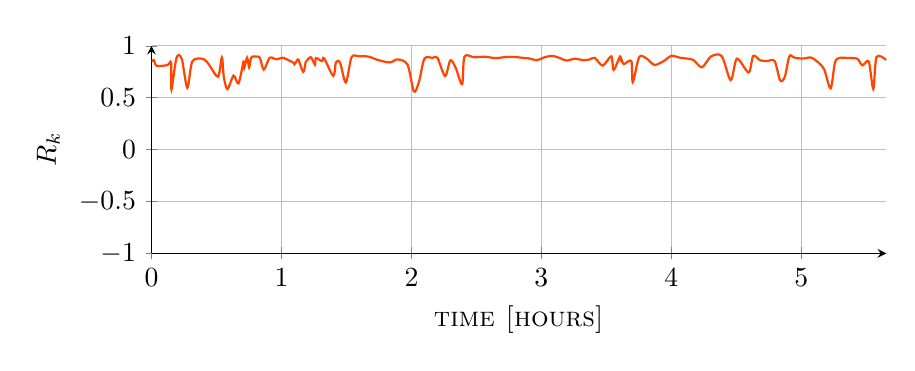
\begin{tikzpicture}
		\begin{axis}[xlabel=\textsc{time [hours]}, ylabel=\textsc{$R_k$}, axis lines=left, grid=major, width=0.9\linewidth, height=12em, ymax=1, ymin=-1]
			\addplot +[mark=none, OrangeRed, thick, smooth] table {
				0.0 0.8499017607375918
				0.005201388888888889 0.852378662692218
				0.01872388888888889 0.8619959035705657
				0.039122500000000004 0.8081875386751143
				0.12099888888888889 0.8136790413488584
				0.1506225 0.835379930314049
				0.15323416666666667 0.5797509210149113
				0.19265333333333334 0.88545646869313
				0.23245472222222222 0.875349212861954
				0.27539138888888887 0.5949374301811404
				0.3144311111111111 0.8516634939571497
				0.40065666666666666 0.8719184759790667
				0.44513861111111114 0.812675233171645
				0.5119047222222222 0.702410187494365
				0.5411605555555555 0.8888170808958313
				0.5560622222222222 0.701015692117206
				0.5843225000000001 0.5822928240857869
				0.6310513888888889 0.7126478609625865
				0.6695008333333333 0.6383178792240444
				0.7079816666666666 0.8485253242406017
				0.7136877777777777 0.7897413089014129
				0.7353455555555556 0.8854571131285263
				0.7509294444444444 0.7932905398699251
				0.762695 0.8688513123110317
				0.7758727777777777 0.8959346935097874
				0.8047269444444444 0.8956314185849666
				0.8336411111111112 0.8851802459919107
				0.8635875 0.7705159423310727
				0.9080608333333333 0.885240463929869
				0.9409074999999999 0.8767293339167576
				0.96428 0.8702500138814218
				1.0105875 0.8844135720644594
				1.0669716666666667 0.8536539705821563
				1.0943486111111111 0.8354535523421599
				1.0996091666666665 0.8229262958951357
				1.1195386111111112 0.8575535920309041
				1.1316161111111112 0.864146475155814
				1.1660975 0.7487939044492513
				1.1830388888888888 0.8179535855662031
				1.184250277777778 0.837531490140278
				1.2251191666666668 0.8911955571873882
				1.25704 0.8172830674116685
				1.2648908333333333 0.8818281831828046
				1.310643611111111 0.8523578912933206
				1.327995277777778 0.8796004521721426
				1.3982180555555557 0.7105659671728104
				1.4191180555555556 0.8416831173443704
				1.4509066666666668 0.8363616891279179
				1.4952791666666667 0.6468657060042918
				1.538858611111111 0.8893350211704111
				1.5948413888888888 0.8988982483419778
				1.6694316666666666 0.8956776942488117
				1.743308888888889 0.8628970183648939
				1.833571388888889 0.840024054817975
				1.8951775 0.8690651746907312
				1.9706180555555557 0.8166481292020238
				2.0181405555555556 0.5608921384442478
				2.0567541666666664 0.6488742781003078
				2.0997475 0.8754557498200528
				2.162766388888889 0.8833190783157384
				2.19959 0.8858824144230281
				2.2584055555555556 0.7087647131399849
				2.2996491666666663 0.8604359410915715
				2.3404305555555553 0.7880710861241802
				2.3898155555555554 0.6300114737639483
				2.4078686111111107 0.8956153599767633
				2.4816091666666664 0.8898941568933093
				2.566015833333333 0.8944911234289498
				2.6461461111111113 0.8816347478032207
				2.7186669444444442 0.8908115570268569
				2.788875 0.8934006976164668
				2.868539722222222 0.8818687097869559
				2.8940633333333334 0.8812027784111317
				2.967833055555556 0.861544199726345
				3.0200341666666666 0.8886083249658839
				3.0846325 0.9024128233661017
				3.1460375000000003 0.8800912516267848
				3.191295 0.8577568249684718
				3.25815 0.8754406578890008
				3.323284166666667 0.8616898006770103
				3.372608333333333 0.8688160897141918
				3.4098591666666667 0.8839809081840996
				3.4711933333333334 0.8094112506898088
				3.5375994444444445 0.8985050606523389
				3.5556733333333335 0.7668440442228425
				3.604652777777778 0.896160128230302
				3.6127369444444444 0.8447180146747196
				3.6153019444444445 0.8719284188878322
				3.6341375 0.8240522573881833
				3.691683611111111 0.8531472161548626
				3.7031358333333335 0.6494700235694065
				3.75157 0.8898715717681602
				3.8054791666666667 0.8808644556241937
				3.8710044444444445 0.8154937630842025
				3.952165 0.8618991703233354
				3.9991166666666667 0.9044990451245236
				4.071107777777778 0.8841926528098764
				4.165429444444444 0.8654101321167339
				4.235024444444444 0.7930484898557203
				4.303297777777778 0.8960844059319205
				4.386959444444445 0.9009538732949663
				4.45666 0.6686945334300403
				4.504651944444444 0.8762804907392239
				4.594435 0.7429692082587519
				4.629792222222222 0.9029514790039695
				4.684983611111111 0.8593762192048625
				4.737556944444445 0.8535757343432511
				4.7944875 0.8530678837205882
				4.836987499999999 0.6667423216748735
				4.872893611111111 0.7016142038258513
				4.907640555555556 0.8996306650670262
				4.942780000000001 0.8877886430737855
				5.005707777777777 0.8763380432493272
				5.073458055555555 0.8864830392995657
				5.129380555555556 0.8409961055980123
				5.176435277777778 0.7706160576398363
				5.225430277777778 0.5893288740683422
				5.258124444444444 0.8360204237746898
				5.291030277777778 0.8829026768534196
				5.362310833333333 0.8821172379216752
				5.430007777777777 0.8754405182592383
				5.470116944444444 0.811989196358322
				5.5185075 0.847746585673361
				5.553746666666667 0.5834548838840395
				5.578719444444444 0.8928589899913557
				5.653522222222223 0.863111294019854
			};
		\end{axis}
	\end{tikzpicture}
	\caption{Hyper-parameters optimization plot for the tool classifier based on random forest.}
	\label{fig:optimization_application_short_random_forest}
\end{figure}
\begin{table}[H]
	\centering
	\begin{tabular}{ll}
		\toprule
		\textsc{hyper-parameter} & \textsc{value}\\
		\midrule
		\verb|criterion| & entropy\\
		\verb|max_depth| & 20\\
		\verb|min_samples_leaf| & 5\\
		\verb|min_samples_split| & 22\\
		\verb|n_estimators| & 417\\
		\bottomrule
	\end{tabular}
	\caption{Optimal hyper-parameters for the tool classifier based on random forest.}
	\label{tab:hyperparameters_application_short_random_forest}
\end{table}
\begin{table}[H]
	\centering
	\begin{tabular}{lrrrr}
		\toprule
		\textsc{statistic} & \textsc{training set} & \textsc{dev set} & \textsc{kts} & \textsc{uts}\\
		\midrule
		samples & 955872 & 119484 & 119485 & 30144\\
		accuracy [$\%$] & 95.716 & 94.977 & 94.953 & 7.680\\
		balanced accuracy [$\%$] & 95.590 & 89.399 & 90.366 & 8.858\\
		precision [$\%$] & 80.233 & 76.446 & 76.447 & 2.624\\
		recall [$\%$] & 95.590 & 89.399 & 90.366 & 2.531\\
		Cohen’s kappa [$\%$] & 91.752 & 90.300 & 90.285 & 3.298\\
		F-score [$\%$] & 85.925 & 81.341 & 81.477 & 2.577\\
		Jaccard score [$\%$] & 77.432 & 71.180 & 71.442 & 1.572\\
		Hamming loss & 0.043 & 0.050 & 0.050 & 0.923\\
		zero-one loss & 0.043 & 0.050 & 0.050 & 0.923\\
		$R_k$ & 0.919 & 0.904 & 0.904 & 0.041\\
		\bottomrule
	\end{tabular}
	\caption{Classification statistics for the tool classifier based on random forest.}
	\label{tab:classification_application_short_random_forest}
\end{table}
\begin{table}[H]
	\centering
\resizebox{\linewidth}{!}{%
	\begin{tabular}{ll|lllllllllll}
	\setlength{\tabcolsep}{2pt}
		 & & \multicolumn{11}{c}{\textsc{inferred}}\\
		 & & \textsc{chrome} & \textsc{curl} & \textsc{edge} & \textsc{firefox} & \textsc{goldeneye} & \textsc{httrack} & \textsc{hulk} & \textsc{rudy} & \textsc{slowloris} & \textsc{wget} & \textsc{wpull}\\
		\midrule
		\multirow{11}{*}{\rotatebox{90}{\textsc{target}}} & \textsc{chrome} & 1999 & 25 & 166 & 113 & 110 & 9 & 12 & 1 & 3 & 14 & 22\\
		 & \textsc{curl} & 1 & 273 & 13 & 3 & 4 & 11 & 0 & 1 & 1 & 12 & 4\\
		 & \textsc{edge} & 73 & 16 & 2717 & 45 & 26 & 9 & 10 & 0 & 1 & 10 & 9\\
		 & \textsc{firefox} & 140 & 17 & 74 & 1588 & 71 & 41 & 17 & 3 & 2 & 16 & 29\\
		 & \textsc{goldeneye} & 1053 & 22 & 159 & 366 & 74967 & 150 & 1511 & 107 & 10 & 31 & 318\\
		 & \textsc{httrack} & 17 & 6 & 4 & 16 & 20 & 1229 & 2 & 0 & 0 & 0 & 4\\
		 & \textsc{hulk} & 409 & 4 & 21 & 49 & 357 & 15 & 28464 & 20 & 0 & 9 & 93\\
		 & \textsc{rudy} & 3 & 0 & 0 & 1 & 7 & 2 & 7 & 321 & 2 & 0 & 5\\
		 & \textsc{slowloris} & 0 & 2 & 1 & 9 & 0 & 20 & 0 & 1 & 1263 & 0 & 3\\
		 & \textsc{wget} & 2 & 4 & 3 & 3 & 12 & 0 & 1 & 1 & 0 & 449 & 7\\
		 & \textsc{wpull} & 2 & 3 & 4 & 2 & 10 & 4 & 0 & 0 & 0 & 3 & 184\\
	\end{tabular}
	}
	\caption{Confusion matrix for the tool classifier based on random forest on the KTS.}
	\label{tab:confusion_application_short_random_forest}
\end{table}
\begin{figure}[H]
	\centering
	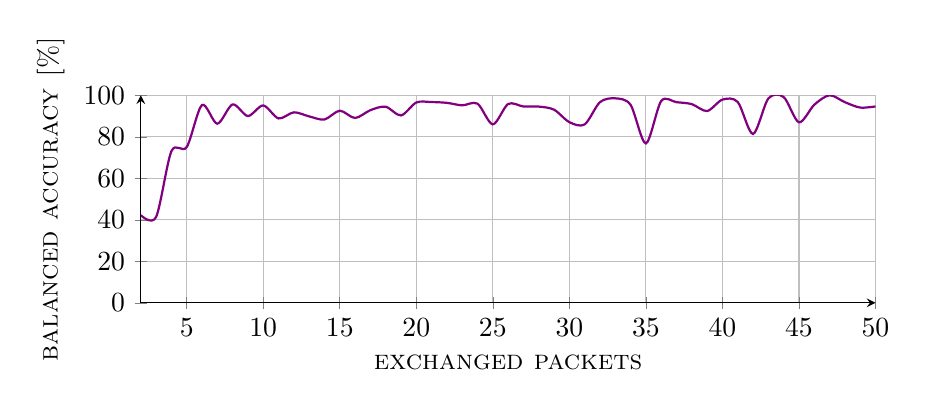
\begin{tikzpicture}
		\begin{axis}[xlabel=\textsc{exchanged packets}, ylabel=\textsc{balanced accuracy [$\%$]}, axis lines=left, grid=major, width=0.9\linewidth, height=12em, ymax=100, ymin=0]
			\addplot +[mark=none, Purple, thick, smooth] table {
				2.0 42.236483206073174
				3.0 41.32632582448161
				4.0 73.00099342702488
				5.0 75.04063244843806
				6.0 95.32490162856543
				7.0 86.30147141729071
				8.0 95.59248784926264
				9.0 90.00302394496346
				10.0 95.09665278556967
				11.0 88.84899058478396
				12.0 91.77924342345011
				13.0 89.8227911237004
				14.0 88.3299129286312
				15.0 92.56720903353572
				16.0 89.04828175725164
				17.0 92.82224468529662
				18.0 94.49274243856053
				19.0 90.28392510079738
				20.0 96.52020944937846
				21.0 96.72752044922068
				22.0 96.35058884466439
				23.0 95.16032713898568
				24.0 95.95751611770172
				25.0 85.98409394485833
				26.0 95.81754796426871
				27.0 94.59315706526641
				28.0 94.54121866941772
				29.0 93.0605180996409
				30.0 87.04758794845003
				31.0 85.95333723445758
				32.0 96.69309054757608
				33.0 98.52292768959435
				34.0 95.38195860820802
				35.0 76.81499570388459
				36.0 97.23789303407138
				37.0 96.65824915824915
				38.0 95.7244008714597
				39.0 92.40151985111662
				40.0 97.91666666666666
				41.0 96.74603174603175
				42.0 81.35802469135804
				43.0 98.47528462314456
				44.0 99.14529914529915
				45.0 86.97448750080329
				46.0 95.43650793650794
				47.0 100.0
				48.0 96.66213151927437
				49.0 94.07407407407408
				50.0 94.61805555555556
			};
		\end{axis}
	\end{tikzpicture}
	\caption{Balanced accuracy vs. exchange packets plot for the tool classifier based on random forest on the KTS.}
	\label{fig:packets_application_short_random_forest}
\end{figure}
\begin{table}[H]
	\centering
	\begin{subtable}{.45\linewidth}
		\centering
	\begin{tabular}{ll}
		\toprule
		\textsc{inferred class} & \textsc{samples}\\
		\midrule
		chrome & 688\\
		curl & 6\\
		edge & 329\\
		firefox & 2315\\
		goldeneye & 405\\
		httrack & 113\\
		hulk & 55\\
		rudy & 37\\
		slowloris & 2\\
		wget & 53\\
		wpull & 2531\\
		\bottomrule
	\end{tabular}
	\caption{Classification of \textsc{firefox-68.0}.}
	\end{subtable}
	\begin{subtable}{.45\linewidth}
		\centering
	\begin{tabular}{ll}
		\toprule
		\textsc{inferred class} & \textsc{samples}\\
		\midrule
		chrome & 348\\
		curl & 41\\
		edge & 262\\
		firefox & 639\\
		goldeneye & 1440\\
		httrack & 186\\
		hulk & 185\\
		rudy & 26\\
		slowloris & 6\\
		wget & 207\\
		wpull & 325\\
		\bottomrule
	\end{tabular}
	\caption{Classification of \textsc{grabsite-2.1.16}.}
	\end{subtable}
	\begin{subtable}{.45\linewidth}
		\centering
	\begin{tabular}{ll}
		\toprule
		\textsc{inferred class} & \textsc{samples}\\
		\midrule
		chrome & 5006\\
		curl & 78\\
		edge & 288\\
		firefox & 1013\\
		goldeneye & 2139\\
		httrack & 182\\
		hulk & 34\\
		rudy & 15\\
		slowloris & 3\\
		wget & 20\\
		wpull & 172\\
		\bottomrule
	\end{tabular}
	\caption{Classification of \textsc{opera-62.0.3331.66}.}
	\end{subtable}
	\begin{subtable}{.45\linewidth}
		\centering
	\begin{tabular}{ll}
		\toprule
		\textsc{inferred class} & \textsc{samples}\\
		\midrule
		chrome & 175\\
		curl & 57\\
		edge & 1831\\
		firefox & 2334\\
		goldeneye & 1032\\
		httrack & 372\\
		hulk & 17\\
		rudy & 4022\\
		slowloris & 39\\
		wget & 39\\
		wpull & 1077\\
		\bottomrule
	\end{tabular}
	\caption{Classification of \textsc{slowhttptest-1.6}.}
	\end{subtable}
	\caption{Classification of unknown tools for the tool classifier based on random forest.}
	\label{tab:unknown_application_short_random_forest}
\end{table}

\begin{figure}[H]
	\centering
	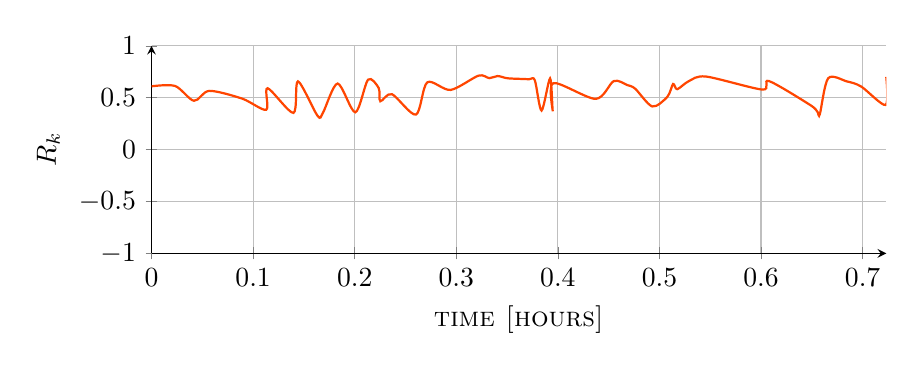
\begin{tikzpicture}
		\begin{axis}[xlabel=\textsc{time [hours]}, ylabel=\textsc{$R_k$}, axis lines=left, grid=major, width=0.9\linewidth, height=12em, ymax=1, ymin=-1]
			\addplot +[mark=none, OrangeRed, thick, smooth] table {
				0.0 0.6097928747463992
				0.02323722222222222 0.6129217596667639
				0.041763611111111106 0.4703741796525676
				0.05695083333333333 0.5659559449855478
				0.08933638888888888 0.49083946217708474
				0.112875 0.3839248315874107
				0.11424583333333334 0.5912762931341725
				0.13971027777777778 0.3535225559525793
				0.14416944444444443 0.65758476919424
				0.16347333333333333 0.3249911079651362
				0.16884305555555557 0.35752147360542386
				0.18322277777777776 0.6363924381979323
				0.20063166666666668 0.3595746041350477
				0.21317527777777778 0.6743027977006054
				0.22363305555555554 0.593351071704001
				0.2252461111111111 0.46589422970395195
				0.23667916666666666 0.5338016730360136
				0.26025722222222225 0.33755169331113033
				0.27146611111111113 0.64794800805626
				0.2943708333333333 0.5749196525598205
				0.32194027777777773 0.7127060139469491
				0.3325061111111111 0.6883212846743243
				0.3406336111111111 0.7086868132977187
				0.34897555555555554 0.6895606230007075
				0.35529333333333335 0.6840343552694009
				0.3716733333333333 0.6777050136213861
				0.37734694444444444 0.667391628950872
				0.38395305555555553 0.3761604603077367
				0.3923538888888889 0.6856641297261536
				0.3949780555555556 0.369087550079868
				0.3956847222222222 0.6405498787099887
				0.4372683333333333 0.48872005894110854
				0.4550363888888889 0.6598688346461978
				0.4682030555555555 0.6222052288545724
				0.4761391666666667 0.5864463418609243
				0.49299499999999996 0.41575258733027903
				0.507818611111111 0.5090080565730162
				0.5134641666666667 0.6325657375201829
				0.51747 0.5818651273777953
				0.5290283333333333 0.660229263534804
				0.5460172222222223 0.7036853324553758
				0.601403888888889 0.5782540089755777
				0.6077822222222222 0.660559335731482
				0.6483358333333333 0.4299531753362494
				0.6557111111111111 0.36127346482174205
				0.6579066666666666 0.3422101975322571
				0.6661291666666667 0.6872665412197645
				0.6844747222222222 0.6571675886232108
				0.69867 0.6071890224266584
				0.7226044444444445 0.4301046366212005
				0.7232886111111111 0.7003922808377742
			};
		\end{axis}
	\end{tikzpicture}
	\caption{Hyper-parameters optimization plot for the tool classifier based on extra-trees.}
	\label{fig:optimization_application_short_extra_trees}
\end{figure}
\begin{table}[H]
	\centering
	\begin{tabular}{ll}
		\toprule
		\textsc{hyper-parameter} & \textsc{value}\\
		\midrule
		\verb|criterion| & entropy\\
		\verb|max_depth| & 20\\
		\verb|min_samples_leaf| & 21\\
		\verb|min_samples_split| & 49\\
		\verb|n_estimators| & 96\\
		\bottomrule
	\end{tabular}
	\caption{Optimal hyper-parameters for the tool classifier based on extra-trees.}
	\label{tab:hyperparameters_application_short_extra_trees}
\end{table}
\begin{table}[H]
	\centering
	\begin{tabular}{lrrrr}
		\toprule
		\textsc{statistic} & \textsc{training set} & \textsc{dev set} & \textsc{kts} & \textsc{uts}\\
		\midrule
		samples & 955872 & 119484 & 119485 & 30144\\
		accuracy [$\%$] & 83.376 & 83.256 & 83.226 & 4.668\\
		balanced accuracy [$\%$] & 69.140 & 66.884 & 66.701 & 5.383\\
		precision [$\%$] & 50.983 & 49.885 & 49.685 & 3.105\\
		recall [$\%$] & 69.140 & 66.884 & 66.701 & 1.538\\
		Cohen’s kappa [$\%$] & 70.282 & 70.017 & 70.042 & 2.396\\
		F-score [$\%$] & 52.837 & 51.522 & 51.257 & 2.057\\
		Jaccard score [$\%$] & 39.406 & 38.294 & 38.123 & 1.202\\
		Hamming loss & 0.166 & 0.167 & 0.168 & 0.953\\
		zero-one loss & 0.166 & 0.167 & 0.168 & 0.953\\
		$R_k$ & 0.713 & 0.710 & 0.711 & 0.030\\
		\bottomrule
	\end{tabular}
	\caption{Classification statistics for the tool classifier based on extra-trees.}
	\label{tab:classification_application_short_extra_trees}
\end{table}
\begin{table}[H]
	\centering
\resizebox{\linewidth}{!}{%
	\begin{tabular}{ll|lllllllllll}
	\setlength{\tabcolsep}{2pt}
		 & & \multicolumn{11}{c}{\textsc{inferred}}\\
		 & & \textsc{chrome} & \textsc{curl} & \textsc{edge} & \textsc{firefox} & \textsc{goldeneye} & \textsc{httrack} & \textsc{hulk} & \textsc{rudy} & \textsc{slowloris} & \textsc{wget} & \textsc{wpull}\\
		\midrule
		\multirow{11}{*}{\rotatebox{90}{\textsc{target}}} & \textsc{chrome} & 1256 & 73 & 208 & 112 & 358 & 126 & 43 & 13 & 153 & 64 & 68\\
		 & \textsc{curl} & 0 & 179 & 22 & 0 & 41 & 38 & 2 & 1 & 26 & 7 & 7\\
		 & \textsc{edge} & 124 & 35 & 2025 & 30 & 103 & 140 & 51 & 10 & 284 & 11 & 103\\
		 & \textsc{firefox} & 204 & 52 & 171 & 837 & 286 & 169 & 27 & 17 & 68 & 63 & 104\\
		 & \textsc{goldeneye} & 92 & 237 & 1084 & 57 & 66908 & 5511 & 1061 & 173 & 2759 & 458 & 354\\
		 & \textsc{httrack} & 17 & 15 & 15 & 14 & 122 & 978 & 1 & 1 & 94 & 13 & 28\\
		 & \textsc{hulk} & 26 & 6 & 431 & 38 & 1496 & 1225 & 25393 & 15 & 641 & 20 & 150\\
		 & \textsc{rudy} & 0 & 2 & 4 & 0 & 32 & 19 & 5 & 249 & 33 & 2 & 2\\
		 & \textsc{slowloris} & 1 & 0 & 2 & 0 & 0 & 35 & 0 & 0 & 1260 & 0 & 1\\
		 & \textsc{wget} & 4 & 18 & 19 & 0 & 40 & 51 & 4 & 3 & 68 & 255 & 20\\
		 & \textsc{wpull} & 1 & 5 & 8 & 1 & 36 & 38 & 0 & 6 & 12 & 3 & 102\\
	\end{tabular}
	}
	\caption{Confusion matrix for the tool classifier based on extra-trees on the KTS.}
	\label{tab:confusion_application_short_extra_trees}
\end{table}
\begin{figure}[H]
	\centering
	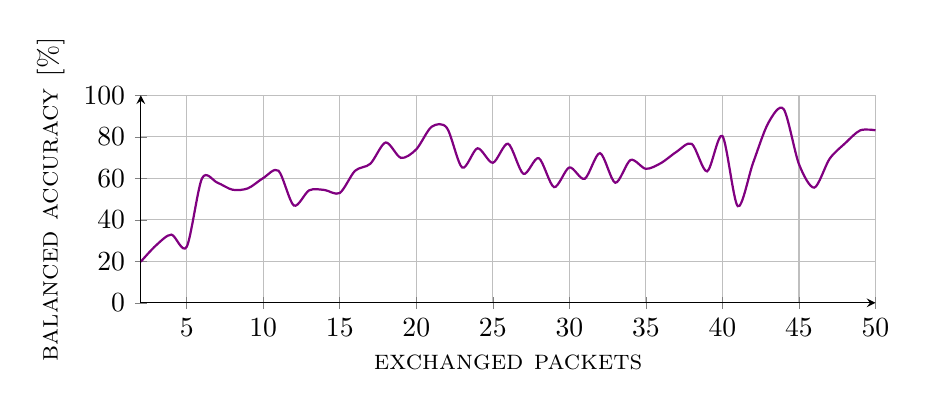
\begin{tikzpicture}
		\begin{axis}[xlabel=\textsc{exchanged packets}, ylabel=\textsc{balanced accuracy [$\%$]}, axis lines=left, grid=major, width=0.9\linewidth, height=12em, ymax=100, ymin=0]
			\addplot +[mark=none, Purple, thick, smooth] table {
				2.0 19.80215827338129
				3.0 27.704762304035384
				4.0 32.85624490428353
				5.0 26.97937261027903
				6.0 59.943742285905486
				7.0 57.91323697307021
				8.0 54.47910122958608
				9.0 55.15588866996144
				10.0 60.11807057046714
				11.0 63.63519726548047
				12.0 46.89928953053374
				13.0 54.195948582925894
				14.0 54.37530452970495
				15.0 52.92425914287415
				16.0 63.61159239814849
				17.0 67.00845207664909
				18.0 77.25086710746453
				19.0 69.82728953382974
				20.0 73.96728270871684
				21.0 84.80611800488667
				22.0 84.28690010149812
				23.0 65.15214866434378
				24.0 74.44803538968412
				25.0 67.47474803130483
				26.0 76.65138213650722
				27.0 62.141781460501065
				28.0 69.71009134808814
				29.0 55.74970635038803
				30.0 65.22850052246604
				31.0 59.750853975439036
				32.0 72.12739316869433
				33.0 57.857026826325075
				34.0 68.83629334013975
				35.0 64.56518789852123
				36.0 67.39366595895258
				37.0 72.76455026455027
				38.0 76.56950237190101
				39.0 63.33694149287865
				40.0 80.36084254143647
				41.0 46.58445153107075
				42.0 67.38067964872089
				43.0 86.71714988187102
				44.0 93.32850840915357
				45.0 66.81720326457167
				46.0 55.505851765993754
				47.0 69.37405241498809
				48.0 76.77132391418107
				49.0 83.09283309283309
				50.0 83.13933829823661
			};
		\end{axis}
	\end{tikzpicture}
	\caption{Balanced accuracy vs. exchange packets plot for the tool classifier based on extra-trees on the KTS.}
	\label{fig:packets_application_short_extra_trees}
\end{figure}
\begin{table}[H]
	\centering
	\begin{subtable}{.45\linewidth}
		\centering
	\begin{tabular}{ll}
		\toprule
		\textsc{inferred class} & \textsc{samples}\\
		\midrule
		chrome & 260\\
		curl & 350\\
		edge & 663\\
		firefox & 1407\\
		goldeneye & 495\\
		httrack & 585\\
		hulk & 2249\\
		rudy & 8\\
		slowloris & 41\\
		wget & 215\\
		wpull & 261\\
		\bottomrule
	\end{tabular}
	\caption{Classification of \textsc{firefox-68.0}.}
	\end{subtable}
	\begin{subtable}{.45\linewidth}
		\centering
	\begin{tabular}{ll}
		\toprule
		\textsc{inferred class} & \textsc{samples}\\
		\midrule
		chrome & 188\\
		curl & 142\\
		edge & 230\\
		firefox & 187\\
		goldeneye & 1097\\
		httrack & 468\\
		hulk & 32\\
		rudy & 33\\
		slowloris & 132\\
		wget & 293\\
		wpull & 863\\
		\bottomrule
	\end{tabular}
	\caption{Classification of \textsc{grabsite-2.1.16}.}
	\end{subtable}
	\begin{subtable}{.45\linewidth}
		\centering
	\begin{tabular}{ll}
		\toprule
		\textsc{inferred class} & \textsc{samples}\\
		\midrule
		chrome & 3498\\
		curl & 412\\
		edge & 494\\
		firefox & 523\\
		goldeneye & 3009\\
		httrack & 354\\
		hulk & 39\\
		rudy & 147\\
		slowloris & 156\\
		wget & 66\\
		wpull & 252\\
		\bottomrule
	\end{tabular}
	\caption{Classification of \textsc{opera-62.0.3331.66}.}
	\end{subtable}
	\begin{subtable}{.45\linewidth}
		\centering
	\begin{tabular}{ll}
		\toprule
		\textsc{inferred class} & \textsc{samples}\\
		\midrule
		chrome & 373\\
		edge & 1458\\
		firefox & 1120\\
		goldeneye & 2033\\
		httrack & 1598\\
		hulk & 61\\
		rudy & 3516\\
		slowloris & 463\\
		wget & 53\\
		wpull & 320\\
		\bottomrule
	\end{tabular}
	\caption{Classification of \textsc{slowhttptest-1.6}.}
	\end{subtable}
	\caption{Classification of unknown tools for the tool classifier based on extra-trees.}
	\label{tab:unknown_application_short_extra_trees}
\end{table}

\begin{figure}[H]
	\centering
	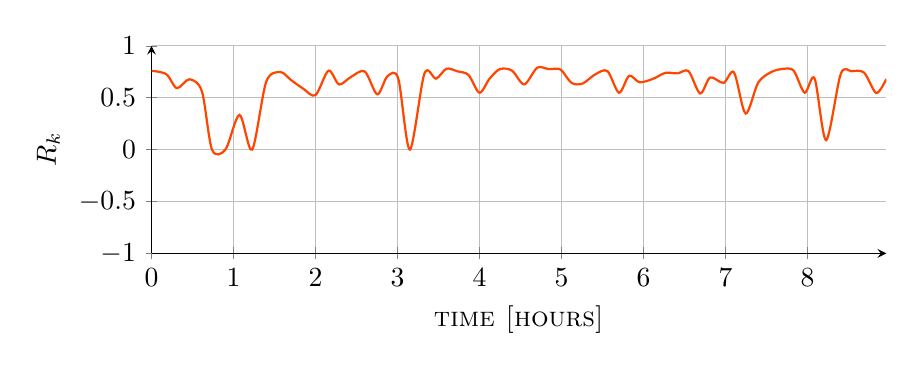
\begin{tikzpicture}
		\begin{axis}[xlabel=\textsc{time [hours]}, ylabel=\textsc{$R_k$}, axis lines=left, grid=major, width=0.9\linewidth, height=12em, ymax=1, ymin=-1]
			\addplot +[mark=none, OrangeRed, thick, smooth] table {
				0.0 0.7591627671109356
				0.1802652777777778 0.7267952609199572
				0.3093427777777778 0.5917755121575778
				0.4630252777777778 0.6778656403246209
				0.6154219444444444 0.5584455131602679
				0.7373394444444444 0.0
				0.9011161111111111 0.0
				1.072718888888889 0.33443777232996097
				1.226907777777778 0.0
				1.3981044444444446 0.6533092503851944
				1.570503888888889 0.7472990217592107
				1.6983436111111112 0.6719069730189826
				1.8506294444444444 0.5865048305008237
				1.998722222222222 0.5242323022094929
				2.1579602777777778 0.7609872938001266
				2.2859269444444443 0.6279563013642984
				2.427344166666667 0.6977177405690668
				2.59862 0.7538603908877894
				2.7524641666666665 0.5321861541755499
				2.874458333333333 0.7050343033058324
				3.008168611111111 0.6861593686382318
				3.1498786111111112 0.0
				3.327237222222222 0.7326719922461692
				3.468863333333333 0.6837695684568718
				3.5966969444444445 0.7795162026761686
				3.730818888888889 0.7538546230854432
				3.864944722222222 0.7191945169384699
				3.9986975 0.5476558535738175
				4.120829444444444 0.682815156429786
				4.2483625 0.7758223921293127
				4.396230555555555 0.7606569840483862
				4.5442052777777775 0.6282912811239846
				4.703128611111111 0.7892139367486724
				4.845043888888889 0.7751591972193846
				4.986085555555555 0.7717879932644219
				5.119824722222222 0.6435192026013359
				5.253292222222222 0.6354769433131923
				5.4114411111111105 0.7254220893463086
				5.559040277777777 0.7563303306968263
				5.700506388888889 0.5474617094154243
				5.822947222222222 0.711325170699539
				5.950933333333333 0.6489784301374649
				6.1145716666666665 0.6817640334927837
				6.266868055555555 0.7395900807944036
				6.414838888888888 0.7343607680067437
				6.547898055555556 0.7555174976696303
				6.689498055555555 0.5403782335500695
				6.811291388888889 0.6947791330380736
				6.974941944444445 0.6426179491715015
				7.1019644444444445 0.7443976268359412
				7.243404444444445 0.3480056207457793
				7.396539166666667 0.6448408004376597
				7.555944722222223 0.747211309417905
				7.702843611111112 0.7779304477358633
				7.830211111111111 0.7601977219374012
				7.963466666666666 0.5480551813985987
				8.085065277777778 0.68518177175519
				8.2253275 0.09117812750092577
				8.4031425 0.7274968638347554
				8.536762222222222 0.7551950379538149
				8.689403333333333 0.7408311533855623
				8.837000833333335 0.5453856644979846
				8.958803611111112 0.6797575804365201
			};
		\end{axis}
	\end{tikzpicture}
	\caption{Hyper-parameters optimization plot for the tool classifier based on neural network.}
	\label{fig:optimization_application_short_neural_network}
\end{figure}
\begin{table}[H]
	\centering
	\begin{tabular}{ll}
		\toprule
		\textsc{hyper-parameter} & \textsc{value}\\
		\midrule
		\verb|lr| & 0.0015639059764891423\\
		\verb|module__layers| & 4\\
		\verb|module__neurons_per_layer| & 196\\
		\verb|module__p| & 0.34048448616373395\\
		\bottomrule
	\end{tabular}
	\caption{Optimal hyper-parameters for the tool classifier based on neural network.}
	\label{tab:hyperparameters_application_short_neural_network}
\end{table}
\begin{table}[H]
	\centering
	\begin{tabular}{lrrrr}
		\toprule
		\textsc{statistic} & \textsc{training set} & \textsc{dev set} & \textsc{kts} & \textsc{uts}\\
		\midrule
		samples & 955872 & 119484 & 119485 & 30144\\
		accuracy [$\%$] & 87.735 & 87.516 & 87.516 & 7.467\\
		balanced accuracy [$\%$] & 81.721 & 79.971 & 80.332 & 8.613\\
		precision [$\%$] & 53.469 & 52.862 & 52.688 & 2.854\\
		recall [$\%$] & 81.721 & 79.971 & 80.332 & 2.461\\
		Cohen’s kappa [$\%$] & 77.740 & 77.340 & 77.379 & 3.560\\
		F-score [$\%$] & 60.582 & 59.641 & 59.479 & 2.643\\
		Jaccard score [$\%$] & 48.020 & 47.214 & 47.164 & 1.621\\
		Hamming loss & 0.123 & 0.125 & 0.125 & 0.925\\
		zero-one loss & 0.123 & 0.125 & 0.125 & 0.925\\
		$R_k$ & 0.785 & 0.782 & 0.782 & 0.044\\
		\bottomrule
	\end{tabular}
	\caption{Classification statistics for the tool classifier based on neural network.}
	\label{tab:classification_application_short_neural_network}
\end{table}
\begin{table}[H]
	\centering
\resizebox{\linewidth}{!}{%
	\begin{tabular}{ll|lllllllllll}
	\setlength{\tabcolsep}{2pt}
		 & & \multicolumn{11}{c}{\textsc{inferred}}\\
		 & & \textsc{chrome} & \textsc{curl} & \textsc{edge} & \textsc{firefox} & \textsc{goldeneye} & \textsc{httrack} & \textsc{hulk} & \textsc{rudy} & \textsc{slowloris} & \textsc{wget} & \textsc{wpull}\\
		\midrule
		\multirow{11}{*}{\rotatebox{90}{\textsc{target}}} & \textsc{chrome} & 1509 & 50 & 204 & 300 & 214 & 42 & 35 & 4 & 2 & 75 & 39\\
		 & \textsc{curl} & 1 & 207 & 14 & 5 & 37 & 14 & 2 & 2 & 0 & 28 & 13\\
		 & \textsc{edge} & 61 & 16 & 2552 & 66 & 36 & 28 & 38 & 10 & 1 & 51 & 57\\
		 & \textsc{firefox} & 165 & 19 & 119 & 1269 & 184 & 80 & 50 & 10 & 1 & 34 & 67\\
		 & \textsc{goldeneye} & 1189 & 313 & 821 & 562 & 67851 & 710 & 3873 & 1273 & 106 & 1176 & 820\\
		 & \textsc{httrack} & 13 & 1 & 37 & 38 & 98 & 1087 & 10 & 1 & 0 & 7 & 6\\
		 & \textsc{hulk} & 367 & 4 & 53 & 48 & 488 & 115 & 27981 & 147 & 0 & 133 & 105\\
		 & \textsc{rudy} & 1 & 0 & 2 & 1 & 5 & 2 & 11 & 306 & 2 & 9 & 9\\
		 & \textsc{slowloris} & 2 & 0 & 0 & 19 & 0 & 15 & 0 & 3 & 1258 & 1 & 1\\
		 & \textsc{wget} & 4 & 15 & 16 & 1 & 17 & 5 & 2 & 6 & 0 & 383 & 33\\
		 & \textsc{wpull} & 1 & 2 & 5 & 5 & 12 & 4 & 3 & 4 & 0 & 10 & 166\\
	\end{tabular}
	}
	\caption{Confusion matrix for the tool classifier based on neural network on the KTS.}
	\label{tab:confusion_application_short_neural_network}
\end{table}
\begin{figure}[H]
	\centering
	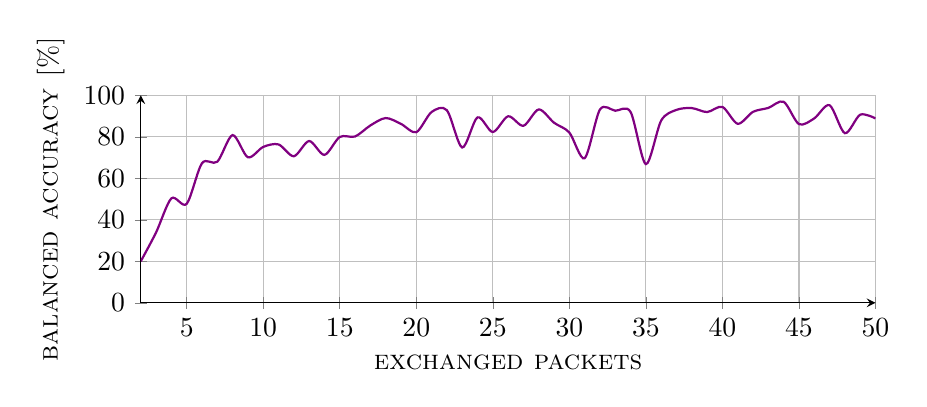
\begin{tikzpicture}
		\begin{axis}[xlabel=\textsc{exchanged packets}, ylabel=\textsc{balanced accuracy [$\%$]}, axis lines=left, grid=major, width=0.9\linewidth, height=12em, ymax=100, ymin=0]
			\addplot +[mark=none, Purple, thick, smooth] table {
				2.0 20.0
				3.0 33.91235880928743
				4.0 50.32953416962991
				5.0 47.700310773849885
				6.0 67.2825853449682
				7.0 67.99250363478195
				8.0 80.81857733214218
				9.0 70.12202750601207
				10.0 75.11646143616304
				11.0 76.31766158693526
				12.0 70.62247079862964
				13.0 77.96409443557297
				14.0 71.28497563286348
				15.0 79.91239720434277
				16.0 80.13903786273931
				17.0 85.45635820926022
				18.0 89.03046280612963
				19.0 86.21513315227138
				20.0 82.21213315697895
				21.0 91.94717394645117
				22.0 92.78642283488155
				23.0 74.83918892760354
				24.0 89.35838098880376
				25.0 82.29096449366435
				26.0 89.87719608916362
				27.0 85.30077692653433
				28.0 93.17949699614131
				29.0 86.75849263644507
				30.0 82.0364420062696
				31.0 69.7030228876702
				32.0 93.136731970867
				33.0 92.55778334725703
				34.0 91.95216906805952
				35.0 66.82471849138516
				36.0 87.8203670003033
				37.0 92.97138047138047
				38.0 93.82796376371476
				39.0 91.91400790764668
				40.0 94.37787753222835
				41.0 86.26070910768419
				42.0 92.02621865852107
				43.0 93.91607383825283
				44.0 96.86242073338848
				45.0 86.09729451834716
				46.0 88.87983354261245
				47.0 95.21767381416504
				48.0 81.74324088609802
				49.0 90.63973063973063
				50.0 88.8389723506249
			};
		\end{axis}
	\end{tikzpicture}
	\caption{Balanced accuracy vs. exchange packets plot for the tool classifier based on neural network on the KTS.}
	\label{fig:packets_application_short_neural_network}
\end{figure}
\begin{table}[H]
	\centering
	\begin{subtable}{.45\linewidth}
		\centering
	\begin{tabular}{ll}
		\toprule
		\textsc{inferred class} & \textsc{samples}\\
		\midrule
		chrome & 339\\
		curl & 0\\
		edge & 717\\
		firefox & 2251\\
		goldeneye & 2612\\
		httrack & 244\\
		hulk & 154\\
		rudy & 1\\
		slowloris & 0\\
		wget & 76\\
		wpull & 140\\
		\bottomrule
	\end{tabular}
	\caption{Classification of \textsc{firefox-68.0}.}
	\end{subtable}
	\begin{subtable}{.45\linewidth}
		\centering
	\begin{tabular}{ll}
		\toprule
		\textsc{inferred class} & \textsc{samples}\\
		\midrule
		chrome & 364\\
		curl & 13\\
		edge & 458\\
		firefox & 558\\
		goldeneye & 670\\
		httrack & 521\\
		hulk & 290\\
		rudy & 133\\
		slowloris & 0\\
		wget & 243\\
		wpull & 415\\
		\bottomrule
	\end{tabular}
	\caption{Classification of \textsc{grabsite-2.1.16}.}
	\end{subtable}
	\begin{subtable}{.45\linewidth}
		\centering
	\begin{tabular}{ll}
		\toprule
		\textsc{inferred class} & \textsc{samples}\\
		\midrule
		chrome & 4097\\
		curl & 138\\
		edge & 134\\
		firefox & 1502\\
		goldeneye & 2342\\
		httrack & 367\\
		hulk & 80\\
		rudy & 29\\
		slowloris & 4\\
		wget & 59\\
		wpull & 198\\
		\bottomrule
	\end{tabular}
	\caption{Classification of \textsc{opera-62.0.3331.66}.}
	\end{subtable}
	\begin{subtable}{.45\linewidth}
		\centering
	\begin{tabular}{ll}
		\toprule
		\textsc{inferred class} & \textsc{samples}\\
		\midrule
		chrome & 1831\\
		curl & 109\\
		edge & 704\\
		firefox & 1323\\
		goldeneye & 270\\
		httrack & 378\\
		hulk & 109\\
		rudy & 4144\\
		slowloris & 338\\
		wget & 640\\
		wpull & 1149\\
		\bottomrule
	\end{tabular}
	\caption{Classification of \textsc{slowhttptest-1.6}.}
	\end{subtable}
	\caption{Classification of unknown tools for the tool classifier based on neural network.}
	\label{tab:unknown_application_short_neural_network}
\end{table}


\subsection*{Tool instance classifiers}

This section reports several statistics and plots about the models for classifying the traffic into tool instances
(e.g. \textsc{goldeneye-2.1}, \textsc{firefox-62.0}, \textsc{hulk-1.0}, \textsc{wget-1.11.4},
\textsc{edge-42.17134.1.0}, \textsc{httrack-3.49.2}, \textsc{chrome-48.0.2564.109}, \textsc{rudy-1.0.0},
\textsc{chrome-68.0.3440.84}, \textsc{firefox-42.0}, \textsc{slowloris-0.1.5}, \textsc{curl-7.55.1},
\textsc{curl-7.61.0}, \textsc{slowloris-0.1.4}, \textsc{wpull-2.0.1} and \textsc{wget-1.19.5}).
\begin{figure}[H]
	\centering
	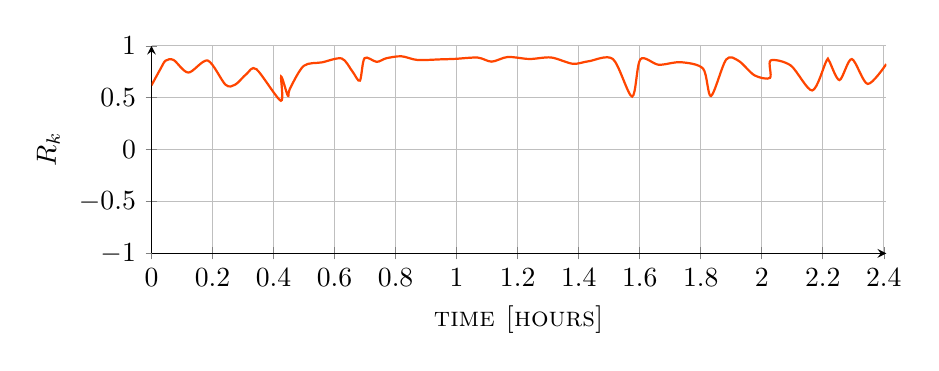
\begin{tikzpicture}
		\begin{axis}[xlabel=\textsc{time [hours]}, ylabel=\textsc{$R_k$}, axis lines=left, grid=major, width=0.9\linewidth, height=12em, ymax=1, ymin=-1]
			\addplot +[mark=none, OrangeRed, thick, smooth] table {
				0.0 0.6197258324124693
				0.029451666666666664 0.7780281900755717
				0.045969444444444445 0.8568861107993396
				0.07251972222222224 0.8631026530981518
				0.1207125 0.7420475867097251
				0.1844713888888889 0.8577557709343541
				0.24249166666666666 0.6252603862875922
				0.27450277777777776 0.6260366430947044
				0.3108925 0.7273702337589893
				0.34354944444444446 0.7752337667775194
				0.42398888888888886 0.4701261443944163
				0.4249991666666667 0.7028196005171105
				0.44684472222222227 0.5185459069092739
				0.45339027777777774 0.5858202814898343
				0.4986922222222222 0.8063907914235793
				0.5586986111111111 0.8406035293608265
				0.6233577777777778 0.8779896652803468
				0.6587488888888889 0.7512991803771675
				0.6829411111111111 0.6644443557745402
				0.6982236111111111 0.8813577541947395
				0.7379925 0.8452468641206403
				0.7694897222222222 0.8800279235961301
				0.8189947222222221 0.8990576196985542
				0.8714033333333334 0.8635864827719679
				0.9476627777777777 0.8695425662520067
				0.9957202777777777 0.8743194040956653
				1.069053888888889 0.8865111572192058
				1.1149888888888888 0.8475163642138497
				1.1675641666666665 0.8924012722543131
				1.2388225000000002 0.873011959272146
				1.3097197222222223 0.8875699734140305
				1.380589722222222 0.8268877009504354
				1.4330180555555554 0.8513901789111508
				1.5124180555555555 0.8719216321290916
				1.5751033333333335 0.5109562981582918
				1.6021605555555556 0.8704321775496318
				1.662174722222222 0.8175957565580481
				1.734423611111111 0.842191507641796
				1.807658888888889 0.7805109775548426
				1.8337208333333335 0.5160690570957521
				1.8833286111111112 0.8678191358901521
				1.9246980555555555 0.8542992991469915
				1.9763775 0.7152918607058433
				2.027149166666667 0.6914182838461037
				2.02891 0.8583944265847114
				2.0952330555555556 0.810100193534843
				2.165444722222222 0.5698351446078668
				2.211320277777778 0.850159971406908
				2.220778055555556 0.8539059120027274
				2.2547605555555554 0.6700373230774287
				2.2951580555555555 0.8725121926486323
				2.3471297222222223 0.6326024759580097
				2.4081411111111115 0.8241075262103797
			};
		\end{axis}
	\end{tikzpicture}
	\caption{Hyper-parameters optimization plot for the tool instance classifier based on random forest.}
	\label{fig:optimization_application_long_random_forest}
\end{figure}
\begin{table}[H]
	\centering
	\begin{tabular}{ll}
		\toprule
		\textsc{hyper-parameter} & \textsc{value}\\
		\midrule
		\verb|criterion| & entropy\\
		\verb|max_depth| & 20\\
		\verb|min_samples_leaf| & 6\\
		\verb|min_samples_split| & 18\\
		\verb|n_estimators| & 314\\
		\bottomrule
	\end{tabular}
	\caption{Optimal hyper-parameters for the tool instance classifier based on random forest.}
	\label{tab:hyperparameters_application_long_random_forest}
\end{table}
\begin{table}[H]
	\centering
	\begin{tabular}{lrrrr}
		\toprule
		\textsc{statistic} & \textsc{training set} & \textsc{dev set} & \textsc{kts} & \textsc{uts}\\
		\midrule
		samples & 955872 & 119484 & 119485 & 30144\\
		accuracy [$\%$] & 95.565 & 94.642 & 94.601 & 0.000\\
		balanced accuracy [$\%$] & 95.196 & 87.183 & 88.021 & 0.000\\
		precision [$\%$] & 79.996 & 74.641 & 75.061 & 0.000\\
		recall [$\%$] & 95.196 & 87.183 & 88.021 & 0.000\\
		Cohen’s kappa [$\%$] & 91.495 & 89.690 & 89.648 & 0.000\\
		F-score [$\%$] & 85.628 & 79.254 & 79.707 & 0.000\\
		Jaccard score [$\%$] & 76.831 & 68.057 & 68.871 & 0.000\\
		Hamming loss & 0.044 & 0.054 & 0.054 & 1.000\\
		zero-one loss & 0.044 & 0.054 & 0.054 & 1.000\\
		$R_k$ & 0.916 & 0.898 & 0.898 & 0.000\\
		\bottomrule
	\end{tabular}
	\caption{Classification statistics for the tool instance classifier based on random forest.}
	\label{tab:classification_application_long_random_forest}
\end{table}
\begin{table}[H]
	\centering
\resizebox{\linewidth}{!}{%
	\begin{tabular}{ll|llllllllllllllll}
	\setlength{\tabcolsep}{2pt}
		 & & \multicolumn{16}{c}{\textsc{inferred}}\\
		 & & \rotatebox{90}{\textsc{ch-48.0}} & \rotatebox{90}{\textsc{ch-68.0}} & \rotatebox{90}{\textsc{cu-7.55.1}} & \rotatebox{90}{\textsc{cu-7.61.0}} & \rotatebox{90}{\textsc{ed-42}} & \rotatebox{90}{\textsc{fi-42.0}} & \rotatebox{90}{\textsc{fi-62.0}} & \rotatebox{90}{\textsc{go-2.1}} & \rotatebox{90}{\textsc{ht-3.49.2}} & \rotatebox{90}{\textsc{hu-1.0}} & \rotatebox{90}{\textsc{ru-1.0.0}} & \rotatebox{90}{\textsc{sl-0.1.4}} & \rotatebox{90}{\textsc{sl-0.1.5}} & \rotatebox{90}{\textsc{wg-1.11.4}} & \rotatebox{90}{\textsc{wg-1.19.5}} & \rotatebox{90}{\textsc{wp-2.0.1}}\\
		\midrule
		\multirow{16}{*}{\rotatebox{90}{\textsc{target}}} & \textsc{ch-48.0} & 1128 & 80 & 14 & 4 & 91 & 18 & 20 & 61 & 4 & 4 & 0 & 0 & 3 & 3 & 10 & 10\\
		 & \textsc{ch-68.0} & 49 & 810 & 7 & 1 & 36 & 18 & 33 & 53 & 6 & 4 & 0 & 0 & 0 & 0 & 1 & 6\\
		 & \textsc{cu-7.55.1} & 0 & 1 & 150 & 6 & 0 & 0 & 3 & 4 & 5 & 0 & 0 & 0 & 1 & 2 & 0 & 0\\
		 & \textsc{cu-7.61.0} & 0 & 0 & 2 & 122 & 9 & 2 & 0 & 0 & 4 & 0 & 1 & 0 & 0 & 2 & 6 & 3\\
		 & \textsc{ed-42} & 75 & 37 & 2 & 21 & 2656 & 32 & 19 & 35 & 9 & 10 & 0 & 0 & 2 & 4 & 6 & 8\\
		 & \textsc{fi-42.0} & 26 & 22 & 9 & 2 & 41 & 646 & 51 & 34 & 12 & 5 & 2 & 0 & 2 & 4 & 3 & 10\\
		 & \textsc{fi-62.0} & 27 & 45 & 9 & 1 & 28 & 46 & 894 & 37 & 17 & 6 & 0 & 0 & 3 & 0 & 5 & 11\\
		 & \textsc{go-2.1} & 114 & 1191 & 50 & 2 & 157 & 74 & 320 & 74802 & 130 & 1459 & 93 & 4 & 5 & 18 & 10 & 265\\
		 & \textsc{ht-3.49.2} & 4 & 15 & 7 & 1 & 7 & 5 & 6 & 23 & 1224 & 2 & 0 & 0 & 1 & 0 & 0 & 3\\
		 & \textsc{hu-1.0} & 35 & 485 & 11 & 0 & 21 & 16 & 53 & 293 & 12 & 28435 & 18 & 0 & 3 & 6 & 0 & 53\\
		 & \textsc{ru-1.0.0} & 3 & 1 & 0 & 1 & 0 & 1 & 0 & 6 & 3 & 7 & 321 & 1 & 0 & 0 & 0 & 4\\
		 & \textsc{sl-0.1.4} & 0 & 0 & 0 & 0 & 0 & 0 & 0 & 0 & 0 & 0 & 1 & 607 & 6 & 0 & 0 & 0\\
		 & \textsc{sl-0.1.5} & 0 & 0 & 4 & 0 & 1 & 6 & 1 & 0 & 13 & 0 & 1 & 48 & 608 & 0 & 0 & 3\\
		 & \textsc{wg-1.11.4} & 2 & 1 & 1 & 2 & 4 & 3 & 0 & 8 & 0 & 1 & 1 & 0 & 0 & 259 & 0 & 1\\
		 & \textsc{wg-1.19.5} & 1 & 0 & 0 & 1 & 0 & 0 & 0 & 0 & 0 & 0 & 0 & 0 & 0 & 0 & 196 & 1\\
		 & \textsc{wp-2.0.1} & 1 & 5 & 1 & 5 & 4 & 4 & 2 & 6 & 3 & 1 & 0 & 0 & 1 & 3 & 0 & 176\\
	\end{tabular}
	}
	\caption{Confusion matrix for the tool instance classifier based on random forest on the KTS (where \textsc{go} = \textsc{goldeneye}, \textsc{fi} = \textsc{firefox}, \textsc{hu} = \textsc{hulk}, \textsc{wg} = \textsc{wget}, \textsc{ed} = \textsc{edge}, \textsc{ht} = \textsc{httrack}, \textsc{ch} = \textsc{chrome}, \textsc{ru} = \textsc{rudy}, \textsc{sl} = \textsc{slowloris}, \textsc{cu} = \textsc{curl} and \textsc{wp} = \textsc{wpull}.}
	\label{tab:confusion_application_long_random_forest}
\end{table}
\begin{figure}[H]
	\centering
	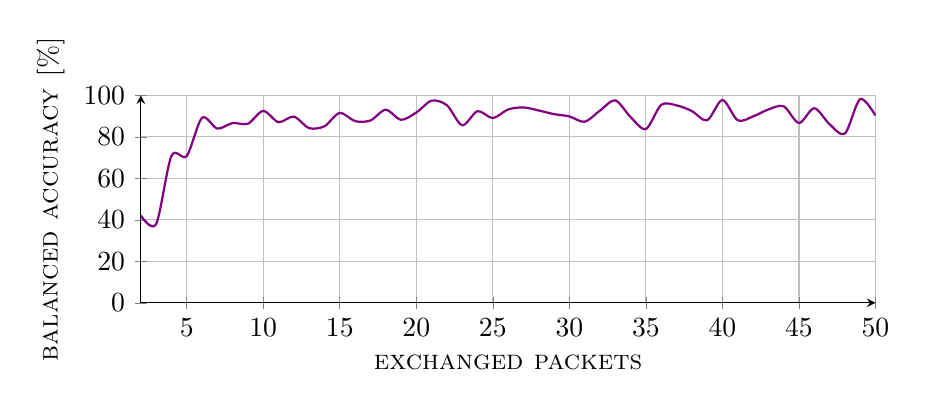
\begin{tikzpicture}
		\begin{axis}[xlabel=\textsc{exchanged packets}, ylabel=\textsc{balanced accuracy [$\%$]}, axis lines=left, grid=major, width=0.9\linewidth, height=12em, ymax=100, ymin=0]
			\addplot +[mark=none, Purple, thick, smooth] table {
				2.0 42.1317694310809
				3.0 37.878439412091915
				4.0 70.72245657277811
				5.0 70.71235573954769
				6.0 89.14889748864925
				7.0 83.96417829326143
				8.0 86.59482838733474
				9.0 86.31159671023984
				10.0 92.4514994816523
				11.0 87.04537601314483
				12.0 89.72490581780448
				13.0 84.17701401779034
				14.0 85.07621759697994
				15.0 91.53221571381057
				16.0 87.53223129389632
				17.0 87.83518209216757
				18.0 93.02528165082997
				19.0 88.20307786098297
				20.0 91.66526326760172
				21.0 97.39631353511471
				22.0 95.21231641921297
				23.0 85.54824154829835
				24.0 92.34650752105459
				25.0 89.00915582986988
				26.0 93.1776735772679
				27.0 94.15026864032708
				28.0 92.67009600897681
				29.0 90.9061436107292
				30.0 89.81332556332556
				31.0 87.2410628790297
				32.0 92.61959341255958
				33.0 97.55291005291005
				34.0 89.51820569703133
				35.0 83.73769748769749
				36.0 95.3997223583211
				37.0 95.14102059556605
				38.0 92.40216853853217
				39.0 87.93947539915281
				40.0 97.72727272727273
				41.0 87.93290043290042
				42.0 89.79166666666666
				43.0 93.14644499469402
				44.0 94.69696969696969
				45.0 86.6338924233661
				46.0 93.7610229276896
				47.0 86.06060606060606
				48.0 81.56043956043956
				49.0 98.18181818181819
				50.0 90.18253968253968
			};
		\end{axis}
	\end{tikzpicture}
	\caption{Balanced accuracy vs. exchange packets plot for the tool instance classifier based on random forest on the KTS.}
	\label{fig:packets_application_long_random_forest}
\end{figure}
\begin{table}[H]
	\centering
	\begin{subtable}{.45\linewidth}
		\centering
	\begin{tabular}{ll}
		\toprule
		\textsc{inferred class} & \textsc{samples}\\
		\midrule
		chrome-48.0.2564.109 & 367\\
		chrome-68.0.3440.84 & 226\\
		curl-7.55.1 & 9\\
		edge-42.17134.1.0 & 356\\
		firefox-42.0 & 607\\
		firefox-62.0 & 1805\\
		goldeneye-2.1 & 377\\
		httrack-3.49.2 & 47\\
		hulk-1.0 & 49\\
		rudy-1.0.0 & 33\\
		slowloris-0.1.5 & 52\\
		wget-1.19.5 & 60\\
		wpull-2.0.1 & 2546\\
		\bottomrule
	\end{tabular}
	\caption{Classification of \textsc{firefox-68.0}.}
	\end{subtable}
	\begin{subtable}{.45\linewidth}
		\centering
	\begin{tabular}{ll}
		\toprule
		\textsc{inferred class} & \textsc{samples}\\
		\midrule
		chrome-48.0.2564.109 & 112\\
		chrome-68.0.3440.84 & 168\\
		curl-7.55.1 & 53\\
		curl-7.61.0 & 2\\
		edge-42.17134.1.0 & 260\\
		firefox-42.0 & 224\\
		firefox-62.0 & 296\\
		goldeneye-2.1 & 1579\\
		httrack-3.49.2 & 164\\
		hulk-1.0 & 223\\
		rudy-1.0.0 & 25\\
		slowloris-0.1.5 & 11\\
		wget-1.11.4 & 84\\
		wget-1.19.5 & 23\\
		wpull-2.0.1 & 441\\
		\bottomrule
	\end{tabular}
	\caption{Classification of \textsc{grabsite-2.1.16}.}
	\end{subtable}
	\begin{subtable}{.45\linewidth}
		\centering
	\begin{tabular}{ll}
		\toprule
		\textsc{inferred class} & \textsc{samples}\\
		\midrule
		chrome-48.0.2564.109 & 2365\\
		chrome-68.0.3440.84 & 2178\\
		curl-7.55.1 & 103\\
		curl-7.61.0 & 5\\
		edge-42.17134.1.0 & 382\\
		firefox-42.0 & 275\\
		firefox-62.0 & 714\\
		goldeneye-2.1 & 2431\\
		httrack-3.49.2 & 231\\
		hulk-1.0 & 35\\
		rudy-1.0.0 & 18\\
		slowloris-0.1.5 & 6\\
		wget-1.11.4 & 12\\
		wget-1.19.5 & 5\\
		wpull-2.0.1 & 190\\
		\bottomrule
	\end{tabular}
	\caption{Classification of \textsc{opera-62.0.3331.66}.}
	\end{subtable}
	\begin{subtable}{.45\linewidth}
		\centering
	\begin{tabular}{ll}
		\toprule
		\textsc{inferred class} & \textsc{samples}\\
		\midrule
		chrome-48.0.2564.109 & 165\\
		chrome-68.0.3440.84 & 27\\
		curl-7.55.1 & 78\\
		curl-7.61.0 & 22\\
		edge-42.17134.1.0 & 1795\\
		firefox-42.0 & 394\\
		firefox-62.0 & 1220\\
		goldeneye-2.1 & 1212\\
		httrack-3.49.2 & 341\\
		hulk-1.0 & 33\\
		rudy-1.0.0 & 4061\\
		slowloris-0.1.4 & 1\\
		slowloris-0.1.5 & 56\\
		wget-1.11.4 & 25\\
		wget-1.19.5 & 8\\
		wpull-2.0.1 & 1557\\
		\bottomrule
	\end{tabular}
	\caption{Classification of \textsc{slowhttptest-1.6}.}
	\end{subtable}
	\caption{Classification of unknown tools for the tool instance classifier based on random forest.}
	\label{tab:unknown_application_long_random_forest}
\end{table}

\begin{figure}[H]
	\centering
	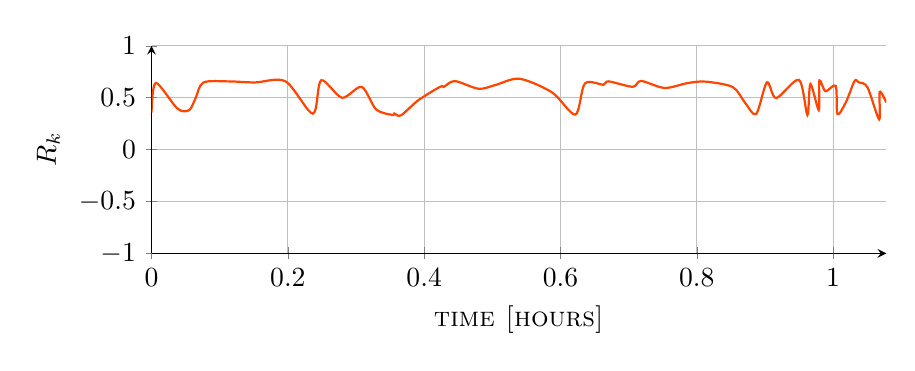
\begin{tikzpicture}
		\begin{axis}[xlabel=\textsc{time [hours]}, ylabel=\textsc{$R_k$}, axis lines=left, grid=major, width=0.9\linewidth, height=12em, ymax=1, ymin=-1]
			\addplot +[mark=none, OrangeRed, thick, smooth] table {
				0.0 0.35546617052879226
				0.006223611111111111 0.6423156409962552
				0.03802861111111111 0.3948780449789209
				0.05518527777777778 0.3799493280869101
				0.06458861111111111 0.4949206401970054
				0.07599277777777778 0.6461311764773638
				0.112955 0.6571725336164813
				0.1514933333333333 0.6468657379384659
				0.1965386111111111 0.6576968364104547
				0.23667472222222222 0.34636345079233055
				0.24885500000000002 0.6675629023801654
				0.27948111111111107 0.4996115206510967
				0.30830555555555555 0.6037966244405408
				0.32964805555555554 0.3861278592165315
				0.3543025 0.33302678719799667
				0.356375 0.34693906848502
				0.36603166666666664 0.3298534993689676
				0.3915313888888889 0.4762810675680167
				0.4238683333333333 0.6065771187486997
				0.4287608333333333 0.6038632136318058
				0.44504305555555557 0.6602064306834037
				0.4797516666666667 0.5862189857657505
				0.5044527777777777 0.6220707533833857
				0.5400936111111111 0.6825126535195893
				0.5878480555555556 0.5502180606125637
				0.6218416666666667 0.33751261002699184
				0.6358591666666666 0.63696760261014
				0.6630413888888889 0.6249804260189633
				0.6704505555555555 0.6575812337656
				0.7060861111111111 0.6050283137635387
				0.7181638888888888 0.6616880607244239
				0.7526675 0.5940724626268492
				0.7866641666666666 0.6412208579892701
				0.8128436111111111 0.6548242872189687
				0.8528219444444445 0.6021817044397049
				0.8707794444444444 0.4511871446602367
				0.8871772222222223 0.34372506384875695
				0.9028527777777777 0.6480821568890699
				0.9165419444444445 0.496500637023338
				0.94991 0.6717195920371388
				0.9622538888888889 0.3333445673634495
				0.9666849999999999 0.6315558619293459
				0.9789675 0.3820189873034296
				0.9799155555555555 0.6655715819369845
				0.9888355555555556 0.562051495977626
				1.003821388888889 0.6135684463196495
				1.0064177777777776 0.34186651764665643
				1.018928611111111 0.45889259641293556
				1.0314227777777778 0.6605144433217767
				1.0375872222222222 0.6477850845274397
				1.0503841666666667 0.6006237048926187
				1.067550277777778 0.2904393253921797
				1.0683886111111112 0.5559489278089268
				1.0779855555555555 0.4539517514956902
			};
		\end{axis}
	\end{tikzpicture}
	\caption{Hyper-parameters optimization plot for the tool instance classifier based on extra-trees.}
	\label{fig:optimization_application_long_extra_trees}
\end{figure}
\begin{table}[H]
	\centering
	\begin{tabular}{ll}
		\toprule
		\textsc{hyper-parameter} & \textsc{value}\\
		\midrule
		\verb|criterion| & gini\\
		\verb|max_depth| & 20\\
		\verb|min_samples_leaf| & 8\\
		\verb|min_samples_split| & 18\\
		\verb|n_estimators| & 417\\
		\bottomrule
	\end{tabular}
	\caption{Optimal hyper-parameters for the tool instance classifier based on extra-trees.}
	\label{tab:hyperparameters_application_long_extra_trees}
\end{table}
\begin{table}[H]
	\centering
	\begin{tabular}{lrrrr}
		\toprule
		\textsc{statistic} & \textsc{training set} & \textsc{dev set} & \textsc{kts} & \textsc{uts}\\
		\midrule
		samples & 955872 & 119484 & 119485 & 30144\\
		accuracy [$\%$] & 80.889 & 80.672 & 80.644 & 0.000\\
		balanced accuracy [$\%$] & 66.162 & 63.546 & 62.533 & 0.000\\
		precision [$\%$] & 44.696 & 42.762 & 42.506 & 0.000\\
		recall [$\%$] & 66.162 & 63.546 & 62.533 & 0.000\\
		Cohen’s kappa [$\%$] & 66.786 & 66.362 & 66.387 & 0.000\\
		F-score [$\%$] & 45.703 & 43.713 & 43.182 & 0.000\\
		Jaccard score [$\%$] & 33.113 & 31.442 & 31.131 & 0.000\\
		Hamming loss & 0.191 & 0.193 & 0.194 & 1.000\\
		zero-one loss & 0.191 & 0.193 & 0.194 & 1.000\\
		$R_k$ & 0.681 & 0.677 & 0.677 & 0.000\\
		\bottomrule
	\end{tabular}
	\caption{Classification statistics for the tool instance classifier based on extra-trees.}
	\label{tab:classification_application_long_extra_trees}
\end{table}
\begin{table}[H]
	\centering
\resizebox{\linewidth}{!}{%
	\begin{tabular}{ll|llllllllllllllll}
	\setlength{\tabcolsep}{2pt}
		 & & \multicolumn{16}{c}{\textsc{inferred}}\\
		 & & \rotatebox{90}{\textsc{ch-48.0}} & \rotatebox{90}{\textsc{ch-68.0}} & \rotatebox{90}{\textsc{cu-7.55.1}} & \rotatebox{90}{\textsc{cu-7.61.0}} & \rotatebox{90}{\textsc{ed-42}} & \rotatebox{90}{\textsc{fi-42.0}} & \rotatebox{90}{\textsc{fi-62.0}} & \rotatebox{90}{\textsc{go-2.1}} & \rotatebox{90}{\textsc{ht-3.49.2}} & \rotatebox{90}{\textsc{hu-1.0}} & \rotatebox{90}{\textsc{ru-1.0.0}} & \rotatebox{90}{\textsc{sl-0.1.4}} & \rotatebox{90}{\textsc{sl-0.1.5}} & \rotatebox{90}{\textsc{wg-1.11.4}} & \rotatebox{90}{\textsc{wg-1.19.5}} & \rotatebox{90}{\textsc{wp-2.0.1}}\\
		\midrule
		\multirow{16}{*}{\rotatebox{90}{\textsc{target}}} & \textsc{ch-48.0} & 721 & 89 & 62 & 5 & 44 & 20 & 23 & 180 & 66 & 0 & 9 & 98 & 48 & 26 & 39 & 20\\
		 & \textsc{ch-68.0} & 92 & 484 & 22 & 4 & 85 & 26 & 20 & 151 & 45 & 32 & 0 & 2 & 6 & 18 & 20 & 17\\
		 & \textsc{cu-7.55.1} & 0 & 0 & 98 & 5 & 2 & 0 & 0 & 34 & 8 & 2 & 1 & 2 & 7 & 13 & 0 & 0\\
		 & \textsc{cu-7.61.0} & 0 & 0 & 2 & 86 & 12 & 0 & 0 & 0 & 18 & 0 & 0 & 13 & 10 & 3 & 3 & 4\\
		 & \textsc{ed-42} & 52 & 93 & 13 & 58 & 1950 & 17 & 11 & 95 & 133 & 47 & 2 & 209 & 126 & 31 & 23 & 56\\
		 & \textsc{fi-42.0} & 45 & 32 & 31 & 12 & 80 & 268 & 95 & 80 & 72 & 3 & 7 & 23 & 42 & 26 & 20 & 33\\
		 & \textsc{fi-62.0} & 70 & 34 & 32 & 6 & 46 & 70 & 498 & 184 & 65 & 3 & 5 & 2 & 20 & 26 & 39 & 29\\
		 & \textsc{go-2.1} & 59 & 72 & 346 & 366 & 901 & 11 & 179 & 64648 & 5382 & 767 & 24 & 2364 & 1052 & 1754 & 660 & 109\\
		 & \textsc{ht-3.49.2} & 8 & 5 & 14 & 1 & 11 & 2 & 4 & 118 & 990 & 1 & 0 & 6 & 73 & 32 & 4 & 29\\
		 & \textsc{hu-1.0} & 2 & 42 & 140 & 52 & 457 & 3 & 171 & 1333 & 1129 & 24964 & 0 & 612 & 52 & 43 & 296 & 145\\
		 & \textsc{ru-1.0.0} & 0 & 0 & 1 & 2 & 6 & 0 & 1 & 29 & 17 & 3 & 236 & 26 & 13 & 10 & 4 & 0\\
		 & \textsc{sl-0.1.4} & 0 & 0 & 0 & 0 & 0 & 0 & 0 & 0 & 0 & 0 & 0 & 525 & 89 & 0 & 0 & 0\\
		 & \textsc{sl-0.1.5} & 0 & 0 & 1 & 0 & 0 & 0 & 0 & 0 & 25 & 0 & 0 & 205 & 453 & 0 & 0 & 1\\
		 & \textsc{wg-1.11.4} & 1 & 1 & 1 & 6 & 5 & 0 & 0 & 22 & 11 & 0 & 0 & 5 & 3 & 212 & 6 & 10\\
		 & \textsc{wg-1.19.5} & 0 & 0 & 1 & 5 & 3 & 0 & 0 & 0 & 21 & 3 & 0 & 30 & 0 & 2 & 132 & 2\\
		 & \textsc{wp-2.0.1} & 2 & 0 & 3 & 9 & 8 & 0 & 1 & 35 & 33 & 0 & 4 & 4 & 7 & 12 & 1 & 93\\
	\end{tabular}
	}
	\caption{Confusion matrix for the tool instance classifier based on extra-trees on the KTS (where \textsc{go} = \textsc{goldeneye}, \textsc{fi} = \textsc{firefox}, \textsc{hu} = \textsc{hulk}, \textsc{wg} = \textsc{wget}, \textsc{ed} = \textsc{edge}, \textsc{ht} = \textsc{httrack}, \textsc{ch} = \textsc{chrome}, \textsc{ru} = \textsc{rudy}, \textsc{sl} = \textsc{slowloris}, \textsc{cu} = \textsc{curl} and \textsc{wp} = \textsc{wpull}.}
	\label{tab:confusion_application_long_extra_trees}
\end{table}
\begin{figure}[H]
	\centering
	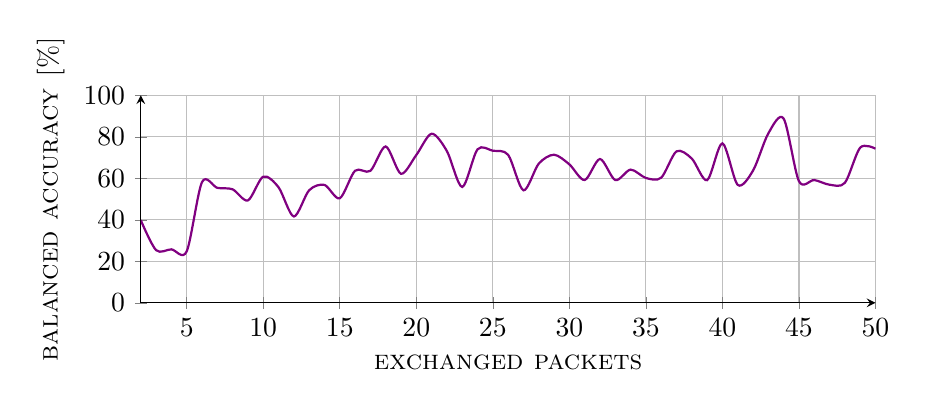
\begin{tikzpicture}
		\begin{axis}[xlabel=\textsc{exchanged packets}, ylabel=\textsc{balanced accuracy [$\%$]}, axis lines=left, grid=major, width=0.9\linewidth, height=12em, ymax=100, ymin=0]
			\addplot +[mark=none, Purple, thick, smooth] table {
				2.0 39.82014388489208
				3.0 25.37890352324433
				4.0 25.76909906125603
				5.0 24.788903279471537
				6.0 58.15627946087795
				7.0 55.39666559459041
				8.0 54.686574440762215
				9.0 49.34978492490254
				10.0 60.79292320332248
				11.0 55.67599410986571
				12.0 41.604812289832005
				13.0 54.23141903388486
				14.0 56.81959372696753
				15.0 50.36032460468392
				16.0 63.641997848681754
				17.0 63.583157700757944
				18.0 75.3311569794528
				19.0 62.184249722921834
				20.0 71.21251008420427
				21.0 81.47267040450839
				22.0 73.0903611677847
				23.0 55.83394591488062
				24.0 73.96223636921825
				25.0 73.27300330434355
				26.0 71.30163084042394
				27.0 54.20413661247863
				28.0 67.06335247629194
				29.0 71.35425758315066
				30.0 66.70200877553819
				31.0 59.16165928354725
				32.0 69.29730230055529
				33.0 59.147276334776336
				34.0 64.18491200130435
				35.0 60.15939307605974
				36.0 60.30143953710832
				37.0 72.99062049062049
				38.0 69.47896640968132
				39.0 59.10328254738712
				40.0 76.82906412188179
				41.0 56.82423906299674
				42.0 63.72685185185185
				43.0 81.66593419157977
				44.0 88.7585532746823
				45.0 58.59311740890688
				46.0 59.153591193821086
				47.0 56.90235690235691
				48.0 57.83272283272284
				49.0 74.77961432506888
				50.0 74.25760021522734
			};
		\end{axis}
	\end{tikzpicture}
	\caption{Balanced accuracy vs. exchange packets plot for the tool instance classifier based on extra-trees on the KTS.}
	\label{fig:packets_application_long_extra_trees}
\end{figure}
\begin{table}[H]
	\centering
	\begin{subtable}{.45\linewidth}
		\centering
	\begin{tabular}{ll}
		\toprule
		\textsc{inferred class} & \textsc{samples}\\
		\midrule
		chrome-48.0.2564.109 & 450\\
		chrome-68.0.3440.84 & 14\\
		curl-7.55.1 & 183\\
		curl-7.61.0 & 58\\
		edge-42.17134.1.0 & 573\\
		firefox-42.0 & 342\\
		firefox-62.0 & 1026\\
		goldeneye-2.1 & 472\\
		httrack-3.49.2 & 596\\
		hulk-1.0 & 2241\\
		rudy-1.0.0 & 22\\
		slowloris-0.1.4 & 2\\
		slowloris-0.1.5 & 23\\
		wget-1.11.4 & 49\\
		wget-1.19.5 & 260\\
		wpull-2.0.1 & 223\\
		\bottomrule
	\end{tabular}
	\caption{Classification of \textsc{firefox-68.0}.}
	\end{subtable}
	\begin{subtable}{.45\linewidth}
		\centering
	\begin{tabular}{ll}
		\toprule
		\textsc{inferred class} & \textsc{samples}\\
		\midrule
		chrome-48.0.2564.109 & 148\\
		chrome-68.0.3440.84 & 24\\
		curl-7.55.1 & 80\\
		curl-7.61.0 & 42\\
		edge-42.17134.1.0 & 217\\
		firefox-42.0 & 46\\
		firefox-62.0 & 156\\
		goldeneye-2.1 & 1039\\
		httrack-3.49.2 & 404\\
		hulk-1.0 & 22\\
		rudy-1.0.0 & 20\\
		slowloris-0.1.4 & 97\\
		slowloris-0.1.5 & 123\\
		wget-1.11.4 & 198\\
		wget-1.19.5 & 170\\
		wpull-2.0.1 & 879\\
		\bottomrule
	\end{tabular}
	\caption{Classification of \textsc{grabsite-2.1.16}.}
	\end{subtable}
	\begin{subtable}{.45\linewidth}
		\centering
	\begin{tabular}{ll}
		\toprule
		\textsc{inferred class} & \textsc{samples}\\
		\midrule
		chrome-48.0.2564.109 & 1913\\
		chrome-68.0.3440.84 & 1672\\
		curl-7.55.1 & 503\\
		curl-7.61.0 & 22\\
		edge-42.17134.1.0 & 432\\
		firefox-42.0 & 192\\
		firefox-62.0 & 220\\
		goldeneye-2.1 & 2978\\
		httrack-3.49.2 & 341\\
		hulk-1.0 & 41\\
		rudy-1.0.0 & 166\\
		slowloris-0.1.4 & 19\\
		slowloris-0.1.5 & 80\\
		wget-1.11.4 & 92\\
		wget-1.19.5 & 81\\
		wpull-2.0.1 & 198\\
		\bottomrule
	\end{tabular}
	\caption{Classification of \textsc{opera-62.0.3331.66}.}
	\end{subtable}
	\begin{subtable}{.45\linewidth}
		\centering
	\begin{tabular}{ll}
		\toprule
		\textsc{inferred class} & \textsc{samples}\\
		\midrule
		chrome-48.0.2564.109 & 271\\
		chrome-68.0.3440.84 & 214\\
		curl-7.55.1 & 6\\
		curl-7.61.0 & 19\\
		edge-42.17134.1.0 & 1473\\
		firefox-42.0 & 211\\
		firefox-62.0 & 581\\
		goldeneye-2.1 & 1965\\
		httrack-3.49.2 & 920\\
		hulk-1.0 & 32\\
		rudy-1.0.0 & 2674\\
		slowloris-0.1.4 & 160\\
		slowloris-0.1.5 & 1592\\
		wget-1.11.4 & 226\\
		wget-1.19.5 & 13\\
		wpull-2.0.1 & 638\\
		\bottomrule
	\end{tabular}
	\caption{Classification of \textsc{slowhttptest-1.6}.}
	\end{subtable}
	\caption{Classification of unknown tools for the tool instance classifier based on extra-trees.}
	\label{tab:unknown_application_long_extra_trees}
\end{table}

\begin{figure}[H]
	\centering
	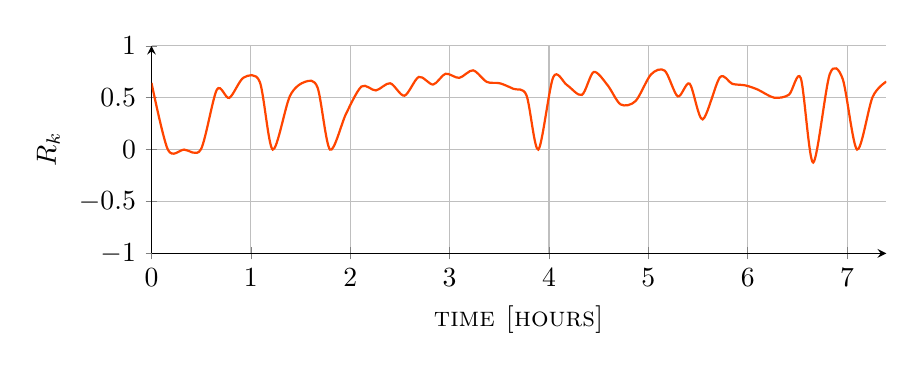
\begin{tikzpicture}
		\begin{axis}[xlabel=\textsc{time [hours]}, ylabel=\textsc{$R_k$}, axis lines=left, grid=major, width=0.9\linewidth, height=12em, ymax=1, ymin=-1]
			\addplot +[mark=none, OrangeRed, thick, smooth] table {
				0.0 0.6424006985899848
				0.16438555555555556 0.0
				0.32832833333333333 0.0
				0.4971713888888889 0.002662851084678322
				0.6574730555555555 0.5769966539062737
				0.78226 0.49821302710772186
				0.9270808333333334 0.6938824543274327
				1.0892377777777777 0.653195733462574
				1.219848888888889 0.0
				1.3924505555555555 0.5153938382140202
				1.546853888888889 0.6533972985358006
				1.6716494444444445 0.5959976721931142
				1.7963813888888889 0.0
				1.9580397222222223 0.3461861842717103
				2.1136838888888887 0.6080391059013339
				2.2577269444444443 0.5701077986178007
				2.40185 0.6393247669119632
				2.5459074999999998 0.5193867696030633
				2.6898524999999998 0.7002048465286903
				2.83405 0.6266763491153108
				2.9585875 0.7304614241854389
				3.096858611111111 0.6910792404855702
				3.2358333333333333 0.7637508046349754
				3.3740705555555555 0.6522848070215357
				3.5046816666666665 0.6391901099196642
				3.642916111111111 0.5851695374619493
				3.773598888888889 0.5238562959054939
				3.893013333333333 0.0
				4.042634722222222 0.6975491939860095
				4.180987222222222 0.622000022367413
				4.331205555555556 0.5268426001384658
				4.4505558333333335 0.747915771020149
				4.59010138888889 0.6203199062273458
				4.721395555555556 0.4352159345869697
				4.871203333333333 0.4672567299467937
				5.027208611111111 0.7248265752760582
				5.165654444444445 0.760051232167923
				5.296549166666667 0.5123718398081342
				5.415977222222223 0.6347507587515153
				5.546555555555555 0.29111494226663426
				5.719841388888889 0.6957064417289627
				5.844479722222222 0.6336917848293709
				5.975399444444444 0.6188097546868678
				6.100168333333333 0.5786263571114891
				6.265580833333334 0.5004639643200648
				6.415464722222222 0.529285574172936
				6.534445833333334 0.6877970950208484
				6.659003333333334 -0.12522726531234257
				6.825095277777778 0.7247316035147445
				6.955981111111111 0.681164253786372
				7.100758888888889 0.0
				7.256611111111111 0.505795978441014
				7.3947899999999995 0.6550998818751443
			};
		\end{axis}
	\end{tikzpicture}
	\caption{Hyper-parameters optimization plot for the tool instance classifier based on neural network.}
	\label{fig:optimization_application_long_neural_network}
\end{figure}
\begin{table}[H]
	\centering
	\begin{tabular}{ll}
		\toprule
		\textsc{hyper-parameter} & \textsc{value}\\
		\midrule
		\verb|lr| & 0.001044660236833224\\
		\verb|module__layers| & 4\\
		\verb|module__neurons_per_layer| & 478\\
		\verb|module__p| & 0.33926635120188525\\
		\bottomrule
	\end{tabular}
	\caption{Optimal hyper-parameters for the tool instance classifier based on neural network.}
	\label{tab:hyperparameters_application_long_neural_network}
\end{table}
\begin{table}[H]
	\centering
	\begin{tabular}{lrrrr}
		\toprule
		\textsc{statistic} & \textsc{training set} & \textsc{dev set} & \textsc{kts} & \textsc{uts}\\
		\midrule
		samples & 955872 & 119484 & 119485 & 30144\\
		accuracy [$\%$] & 83.050 & 82.687 & 82.649 & 0.000\\
		balanced accuracy [$\%$] & 79.137 & 76.554 & 76.767 & 0.000\\
		precision [$\%$] & 45.881 & 44.808 & 44.725 & 0.000\\
		recall [$\%$] & 79.137 & 76.554 & 76.767 & 0.000\\
		Cohen’s kappa [$\%$] & 70.892 & 70.285 & 70.290 & 0.000\\
		F-score [$\%$] & 50.890 & 49.582 & 49.411 & 0.000\\
		Jaccard score [$\%$] & 38.186 & 37.084 & 36.897 & 0.000\\
		Hamming loss & 0.170 & 0.173 & 0.174 & 1.000\\
		zero-one loss & 0.170 & 0.173 & 0.174 & 1.000\\
		$R_k$ & 0.724 & 0.719 & 0.719 & 0.000\\
		\bottomrule
	\end{tabular}
	\caption{Classification statistics for the tool instance classifier based on neural network.}
	\label{tab:classification_application_long_neural_network}
\end{table}
\begin{table}[H]
	\centering
\resizebox{\linewidth}{!}{%
	\begin{tabular}{ll|llllllllllllllll}
	\setlength{\tabcolsep}{2pt}
		 & & \multicolumn{16}{c}{\textsc{inferred}}\\
		 & & \rotatebox{90}{\textsc{ch-48.0}} & \rotatebox{90}{\textsc{ch-68.0}} & \rotatebox{90}{\textsc{cu-7.55.1}} & \rotatebox{90}{\textsc{cu-7.61.0}} & \rotatebox{90}{\textsc{ed-42}} & \rotatebox{90}{\textsc{fi-42.0}} & \rotatebox{90}{\textsc{fi-62.0}} & \rotatebox{90}{\textsc{go-2.1}} & \rotatebox{90}{\textsc{ht-3.49.2}} & \rotatebox{90}{\textsc{hu-1.0}} & \rotatebox{90}{\textsc{ru-1.0.0}} & \rotatebox{90}{\textsc{sl-0.1.4}} & \rotatebox{90}{\textsc{sl-0.1.5}} & \rotatebox{90}{\textsc{wg-1.11.4}} & \rotatebox{90}{\textsc{wg-1.19.5}} & \rotatebox{90}{\textsc{wp-2.0.1}}\\
		\midrule
		\multirow{16}{*}{\rotatebox{90}{\textsc{target}}} & \textsc{ch-48.0} & 832 & 178 & 26 & 14 & 91 & 57 & 78 & 43 & 16 & 6 & 22 & 0 & 2 & 8 & 41 & 36\\
		 & \textsc{ch-68.0} & 60 & 716 & 25 & 1 & 40 & 23 & 80 & 45 & 7 & 8 & 1 & 0 & 2 & 3 & 1 & 12\\
		 & \textsc{cu-7.55.1} & 0 & 2 & 133 & 5 & 0 & 1 & 1 & 6 & 11 & 0 & 0 & 0 & 1 & 6 & 0 & 6\\
		 & \textsc{cu-7.61.0} & 0 & 0 & 0 & 121 & 3 & 1 & 0 & 1 & 6 & 0 & 2 & 0 & 0 & 3 & 12 & 2\\
		 & \textsc{ed-42} & 38 & 77 & 2 & 117 & 2395 & 30 & 40 & 19 & 39 & 33 & 10 & 0 & 1 & 14 & 62 & 39\\
		 & \textsc{fi-42.0} & 25 & 55 & 5 & 16 & 47 & 437 & 155 & 19 & 56 & 5 & 6 & 0 & 4 & 4 & 7 & 28\\
		 & \textsc{fi-62.0} & 18 & 98 & 36 & 2 & 28 & 68 & 752 & 39 & 35 & 6 & 2 & 0 & 6 & 5 & 11 & 23\\
		 & \textsc{go-2.1} & 132 & 1922 & 2542 & 50 & 598 & 123 & 1033 & 63582 & 1334 & 2713 & 1230 & 5 & 45 & 993 & 719 & 1673\\
		 & \textsc{ht-3.49.2} & 5 & 17 & 22 & 1 & 13 & 7 & 24 & 37 & 1150 & 1 & 1 & 0 & 4 & 5 & 3 & 8\\
		 & \textsc{hu-1.0} & 2 & 573 & 76 & 15 & 60 & 20 & 474 & 264 & 123 & 26812 & 287 & 0 & 2 & 23 & 431 & 279\\
		 & \textsc{ru-1.0.0} & 2 & 0 & 1 & 0 & 1 & 1 & 0 & 1 & 5 & 9 & 312 & 2 & 0 & 7 & 0 & 7\\
		 & \textsc{sl-0.1.4} & 0 & 0 & 0 & 0 & 0 & 0 & 0 & 0 & 0 & 0 & 2 & 538 & 74 & 0 & 0 & 0\\
		 & \textsc{sl-0.1.5} & 0 & 0 & 0 & 1 & 0 & 5 & 0 & 0 & 27 & 0 & 1 & 248 & 402 & 0 & 1 & 0\\
		 & \textsc{wg-1.11.4} & 0 & 2 & 2 & 7 & 2 & 1 & 1 & 13 & 8 & 0 & 5 & 0 & 0 & 228 & 2 & 12\\
		 & \textsc{wg-1.19.5} & 0 & 0 & 0 & 6 & 4 & 0 & 0 & 1 & 0 & 0 & 0 & 0 & 0 & 0 & 185 & 3\\
		 & \textsc{wp-2.0.1} & 1 & 8 & 2 & 6 & 5 & 3 & 0 & 3 & 9 & 0 & 5 & 0 & 1 & 8 & 3 & 158\\
	\end{tabular}
	}
	\caption{Confusion matrix for the tool instance classifier based on neural network on the KTS (where \textsc{go} = \textsc{goldeneye}, \textsc{fi} = \textsc{firefox}, \textsc{hu} = \textsc{hulk}, \textsc{wg} = \textsc{wget}, \textsc{ed} = \textsc{edge}, \textsc{ht} = \textsc{httrack}, \textsc{ch} = \textsc{chrome}, \textsc{ru} = \textsc{rudy}, \textsc{sl} = \textsc{slowloris}, \textsc{cu} = \textsc{curl} and \textsc{wp} = \textsc{wpull}.}
	\label{tab:confusion_application_long_neural_network}
\end{table}
\begin{figure}[H]
	\centering
	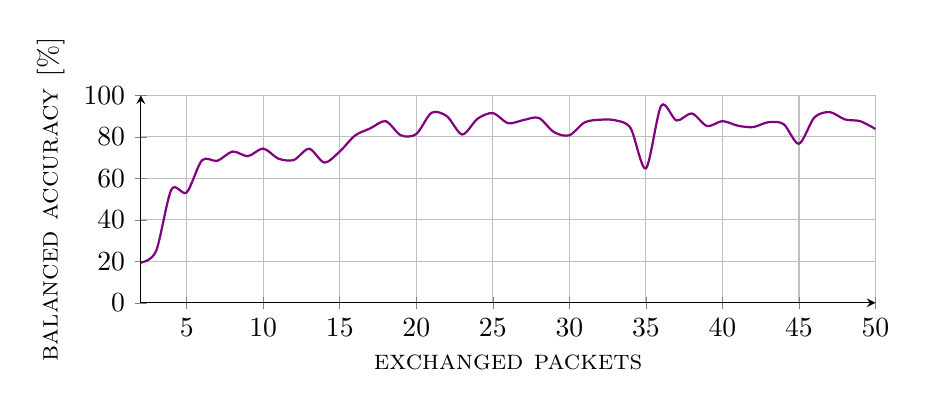
\begin{tikzpicture}
		\begin{axis}[xlabel=\textsc{exchanged packets}, ylabel=\textsc{balanced accuracy [$\%$]}, axis lines=left, grid=major, width=0.9\linewidth, height=12em, ymax=100, ymin=0]
			\addplot +[mark=none, Purple, thick, smooth] table {
				2.0 19.388489208633093
				3.0 24.927869503834874
				4.0 54.527301974595844
				5.0 53.21632886576043
				6.0 68.69625533948522
				7.0 68.42575442351546
				8.0 72.89481847087215
				9.0 70.65940611564585
				10.0 74.31965688045608
				11.0 69.44816884349297
				12.0 68.8225610389293
				13.0 74.24490208322682
				14.0 67.57030596943603
				15.0 72.92575135124757
				16.0 80.61891800686035
				17.0 84.07229893610622
				18.0 87.52780868395364
				19.0 80.67324879954728
				20.0 81.32962410281255
				21.0 91.59309889261436
				22.0 89.90125251023105
				23.0 81.09421371942203
				24.0 88.68005235791361
				25.0 91.4055817405376
				26.0 86.55881657783281
				27.0 88.055203651009
				28.0 89.09556349851754
				29.0 82.20725251502759
				30.0 80.72908953791307
				31.0 86.94967499363247
				32.0 88.20552035039813
				33.0 87.93590668590669
				34.0 84.16668833094546
				35.0 64.75837434170768
				36.0 94.97917687408133
				37.0 87.83451397087761
				38.0 91.25385083681643
				39.0 85.16938714171751
				40.0 87.55483006864222
				41.0 85.34712214346636
				42.0 84.66280068728521
				43.0 87.02711587041266
				44.0 86.08504398826979
				45.0 76.63839084891717
				46.0 89.2606276226966
				47.0 91.91210349105087
				48.0 88.36223036223036
				49.0 87.50688705234158
				50.0 83.741861716438
			};
		\end{axis}
	\end{tikzpicture}
	\caption{Balanced accuracy vs. exchange packets plot for the tool instance classifier based on neural network on the KTS.}
	\label{fig:packets_application_long_neural_network}
\end{figure}
\begin{table}[H]
	\centering
	\begin{subtable}{.45\linewidth}
		\centering
	\begin{tabular}{ll}
		\toprule
		\textsc{inferred class} & \textsc{samples}\\
		\midrule
		chrome-48.0.2564.109 & 142\\
		chrome-68.0.3440.84 & 336\\
		curl-7.55.1 & 62\\
		curl-7.61.0 & 3\\
		edge-42.17134.1.0 & 454\\
		firefox-42.0 & 660\\
		firefox-62.0 & 1651\\
		goldeneye-2.1 & 2386\\
		httrack-3.49.2 & 351\\
		hulk-1.0 & 62\\
		rudy-1.0.0 & 60\\
		slowloris-0.1.4 & 0\\
		slowloris-0.1.5 & 75\\
		wget-1.11.4 & 5\\
		wget-1.19.5 & 96\\
		wpull-2.0.1 & 191\\
		\bottomrule
	\end{tabular}
	\caption{Classification of \textsc{firefox-68.0}.}
	\end{subtable}
	\begin{subtable}{.45\linewidth}
		\centering
	\begin{tabular}{ll}
		\toprule
		\textsc{inferred class} & \textsc{samples}\\
		\midrule
		chrome-48.0.2564.109 & 210\\
		chrome-68.0.3440.84 & 321\\
		curl-7.55.1 & 47\\
		curl-7.61.0 & 19\\
		edge-42.17134.1.0 & 673\\
		firefox-42.0 & 139\\
		firefox-62.0 & 439\\
		goldeneye-2.1 & 480\\
		httrack-3.49.2 & 312\\
		hulk-1.0 & 121\\
		rudy-1.0.0 & 240\\
		slowloris-0.1.4 & 0\\
		slowloris-0.1.5 & 9\\
		wget-1.11.4 & 99\\
		wget-1.19.5 & 201\\
		wpull-2.0.1 & 355\\
		\bottomrule
	\end{tabular}
	\caption{Classification of \textsc{grabsite-2.1.16}.}
	\end{subtable}
	\begin{subtable}{.45\linewidth}
		\centering
	\begin{tabular}{ll}
		\toprule
		\textsc{inferred class} & \textsc{samples}\\
		\midrule
		chrome-48.0.2564.109 & 1636\\
		chrome-68.0.3440.84 & 3446\\
		curl-7.55.1 & 509\\
		curl-7.61.0 & 8\\
		edge-42.17134.1.0 & 75\\
		firefox-42.0 & 281\\
		firefox-62.0 & 1091\\
		goldeneye-2.1 & 1292\\
		httrack-3.49.2 & 322\\
		hulk-1.0 & 26\\
		rudy-1.0.0 & 20\\
		slowloris-0.1.4 & 0\\
		slowloris-0.1.5 & 7\\
		wget-1.11.4 & 45\\
		wget-1.19.5 & 28\\
		wpull-2.0.1 & 164\\
		\bottomrule
	\end{tabular}
	\caption{Classification of \textsc{opera-62.0.3331.66}.}
	\end{subtable}
	\begin{subtable}{.45\linewidth}
		\centering
	\begin{tabular}{ll}
		\toprule
		\textsc{inferred class} & \textsc{samples}\\
		\midrule
		chrome-48.0.2564.109 & 920\\
		chrome-68.0.3440.84 & 239\\
		curl-7.55.1 & 33\\
		curl-7.61.0 & 71\\
		edge-42.17134.1.0 & 1022\\
		firefox-42.0 & 473\\
		firefox-62.0 & 1262\\
		goldeneye-2.1 & 100\\
		httrack-3.49.2 & 735\\
		hulk-1.0 & 61\\
		rudy-1.0.0 & 4359\\
		slowloris-0.1.4 & 9\\
		slowloris-0.1.5 & 3\\
		wget-1.11.4 & 405\\
		wget-1.19.5 & 129\\
		wpull-2.0.1 & 1174\\
		\bottomrule
	\end{tabular}
	\caption{Classification of \textsc{slowhttptest-1.6}.}
	\end{subtable}
	\caption{Classification of unknown tools for the tool instance classifier based on neural network.}
	\label{tab:unknown_application_long_neural_network}
\end{table}

\end{document}
